\clearpage
\makeatletter
\efloat@restorefloats
\makeatother


\begin{appendix}
\section{}
\renewcommand{\appendixname}{Supplementary Materials}
\renewcommand{\thefigure}{S\arabic{figure}} \setcounter{figure}{0}
\renewcommand{\thetable}{S\arabic{table}} \setcounter{table}{0}
\renewcommand{\theequation}{S\arabic{table}} \setcounter{equation}{0}
\graphicspath{{"../Documents/Tables and Figures/"}}

\begin{figure}
\centering
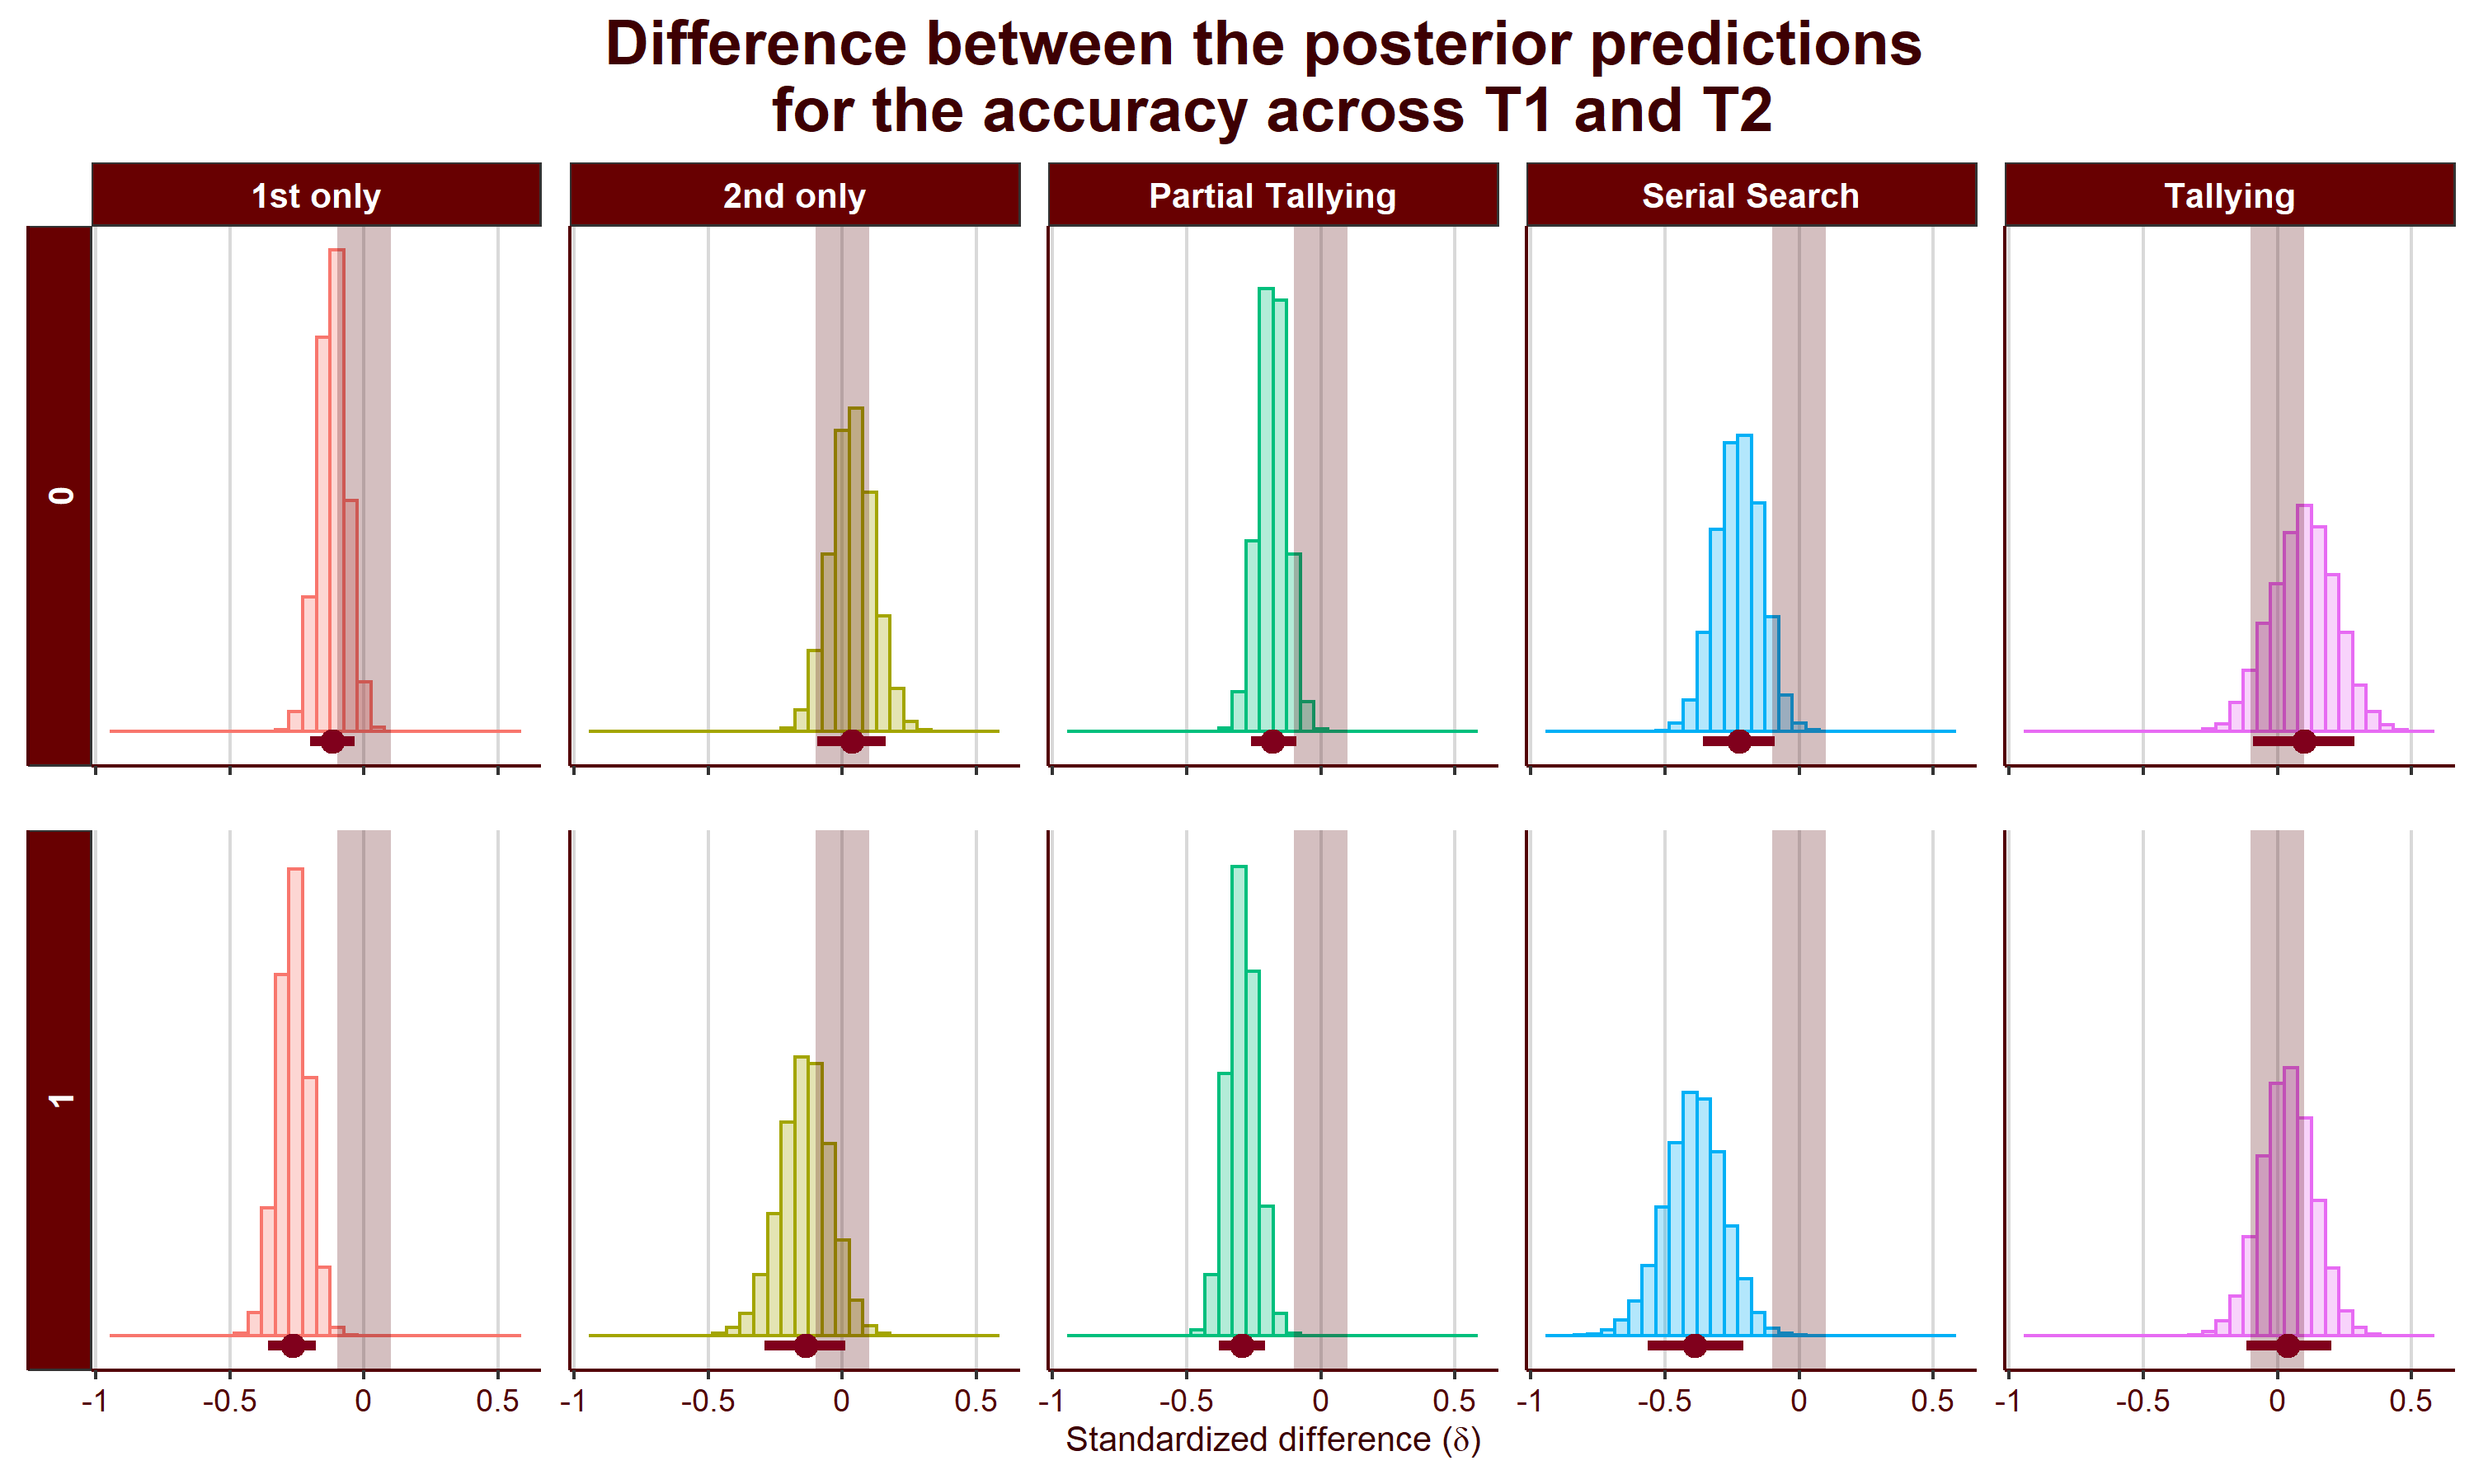
\includegraphics{C:/Users/rerr_/Google Drive/Graduate/Lab/Studies/MultiCue_Probabilistic/Stages/Shifted Weights/Eye Tracking/Analysis/Figures/SB1_performance_change.png}
\caption{(\#fig:performance-change)Difference in performance (as
standardized difference) across testing phases for the different
decision groups. The horizontal red bar represents the 0.89 HDI. The
shaded area highlights the ROPE used in these comparisons}
\end{figure}

\begin{figure}
\centering
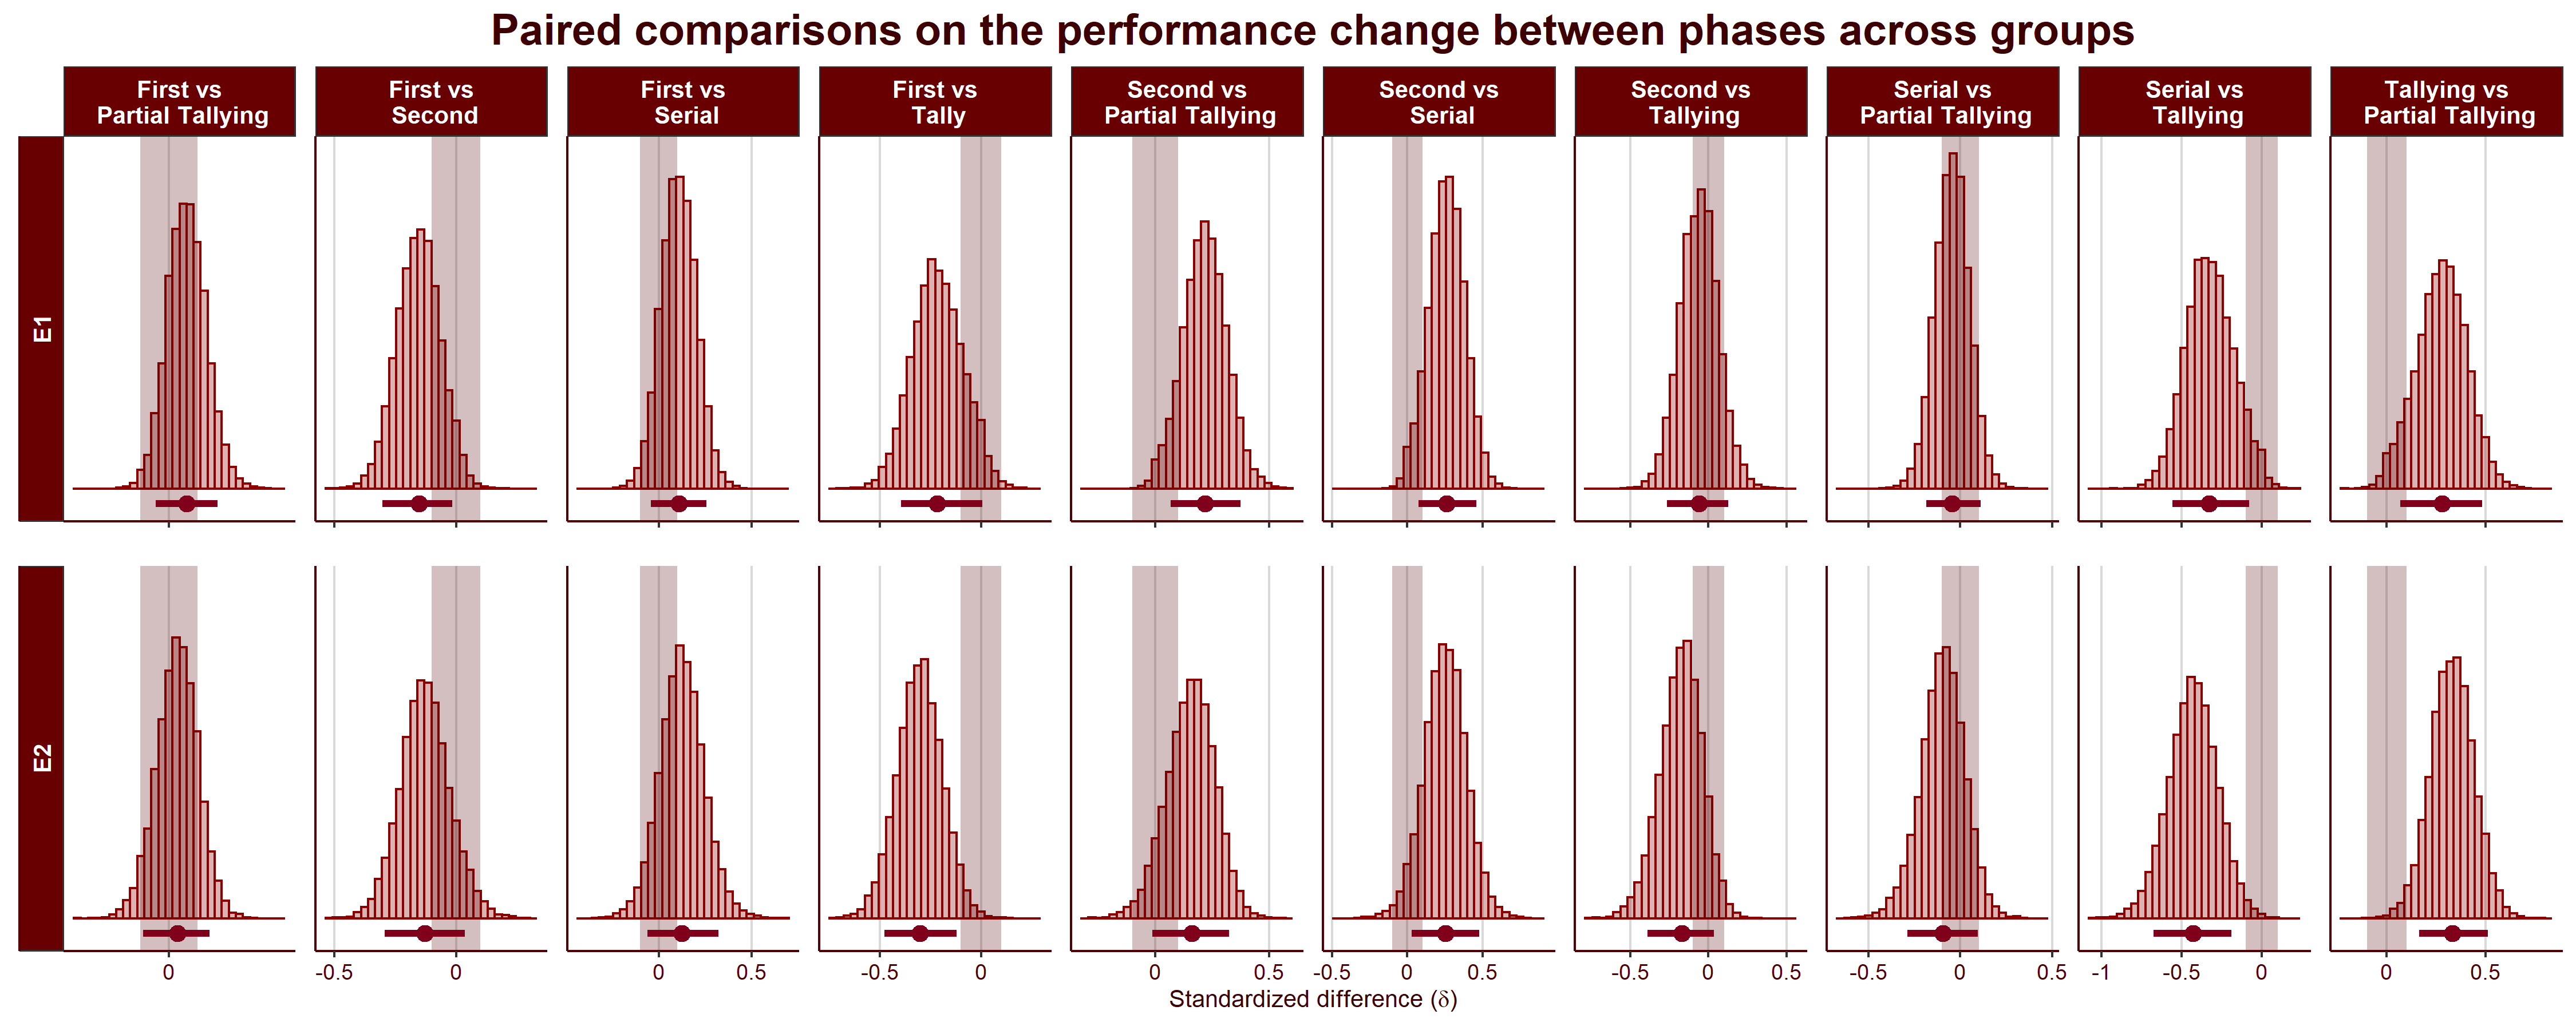
\includegraphics{C:/Users/rerr_/Google Drive/Graduate/Lab/Studies/MultiCue_Probabilistic/Stages/Shifted Weights/Eye Tracking/Analysis/Figures/SB2_performance_change_group.png}
\caption{(\#fig:performance-change-group)Paired comparisons between
groupds on their performance change across phases. The horizontal red
bar represents the 0.89 HDI. The shaded area highlights the ROPE used in
these comparisons}
\end{figure}

\begin{figure}
\centering
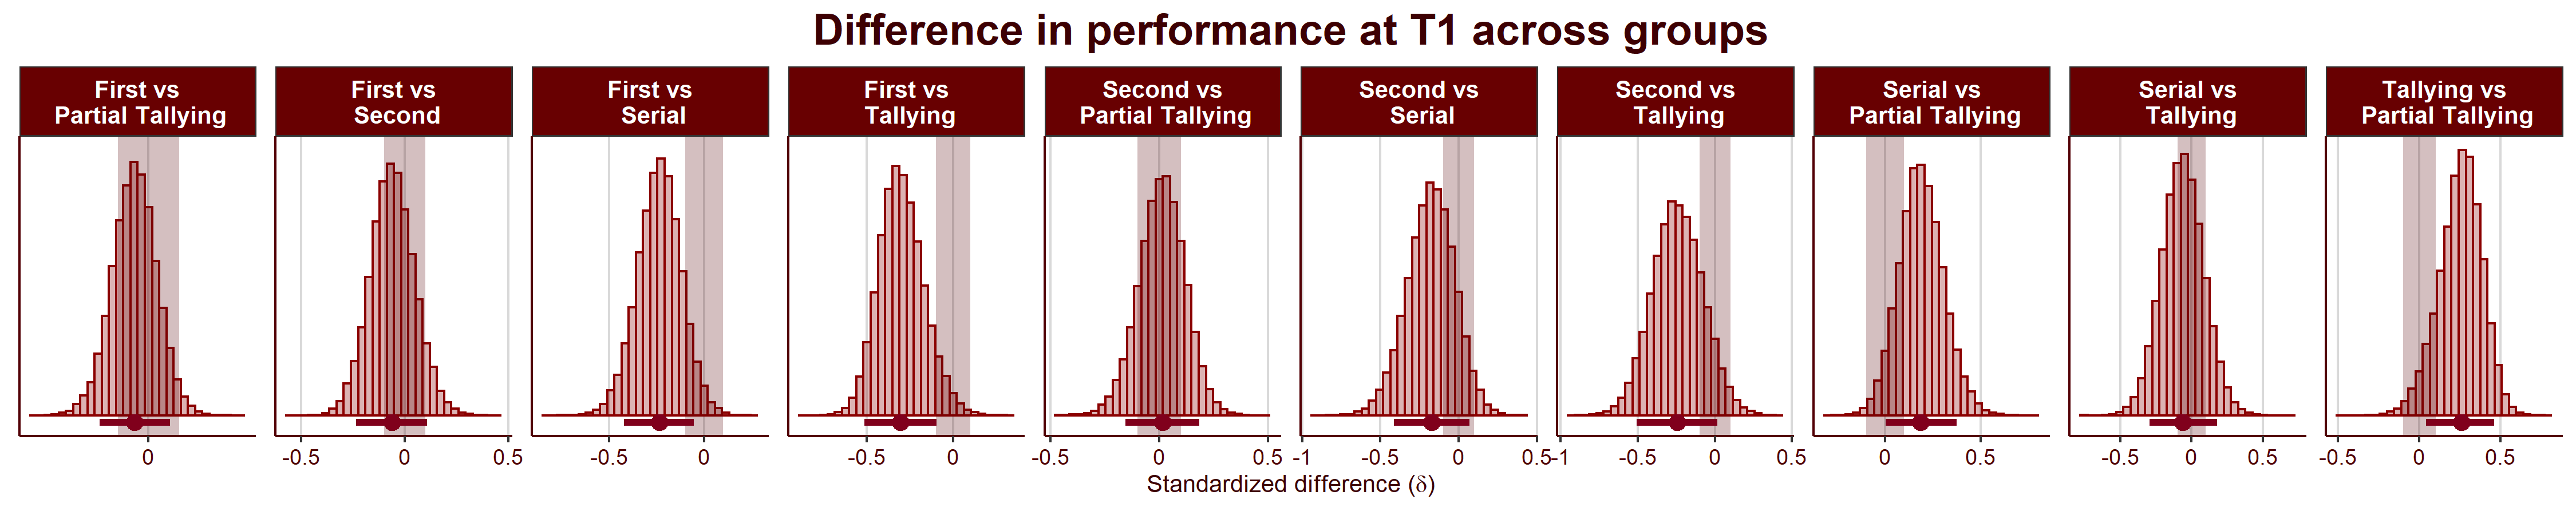
\includegraphics{C:/Users/rerr_/Google Drive/Graduate/Lab/Studies/MultiCue_Probabilistic/Stages/Shifted Weights/Eye Tracking/Analysis/Figures/SB3_performance_T1.png}
\caption{(\#fig:performance-T1)Difference in performance (as
standardized difference) at T1 across decision groups. The horizontal
red bar represents the 0.89 HDI. The shaded area highlights the ROPE
used in these comparisons}
\end{figure}

\begin{figure}
\centering
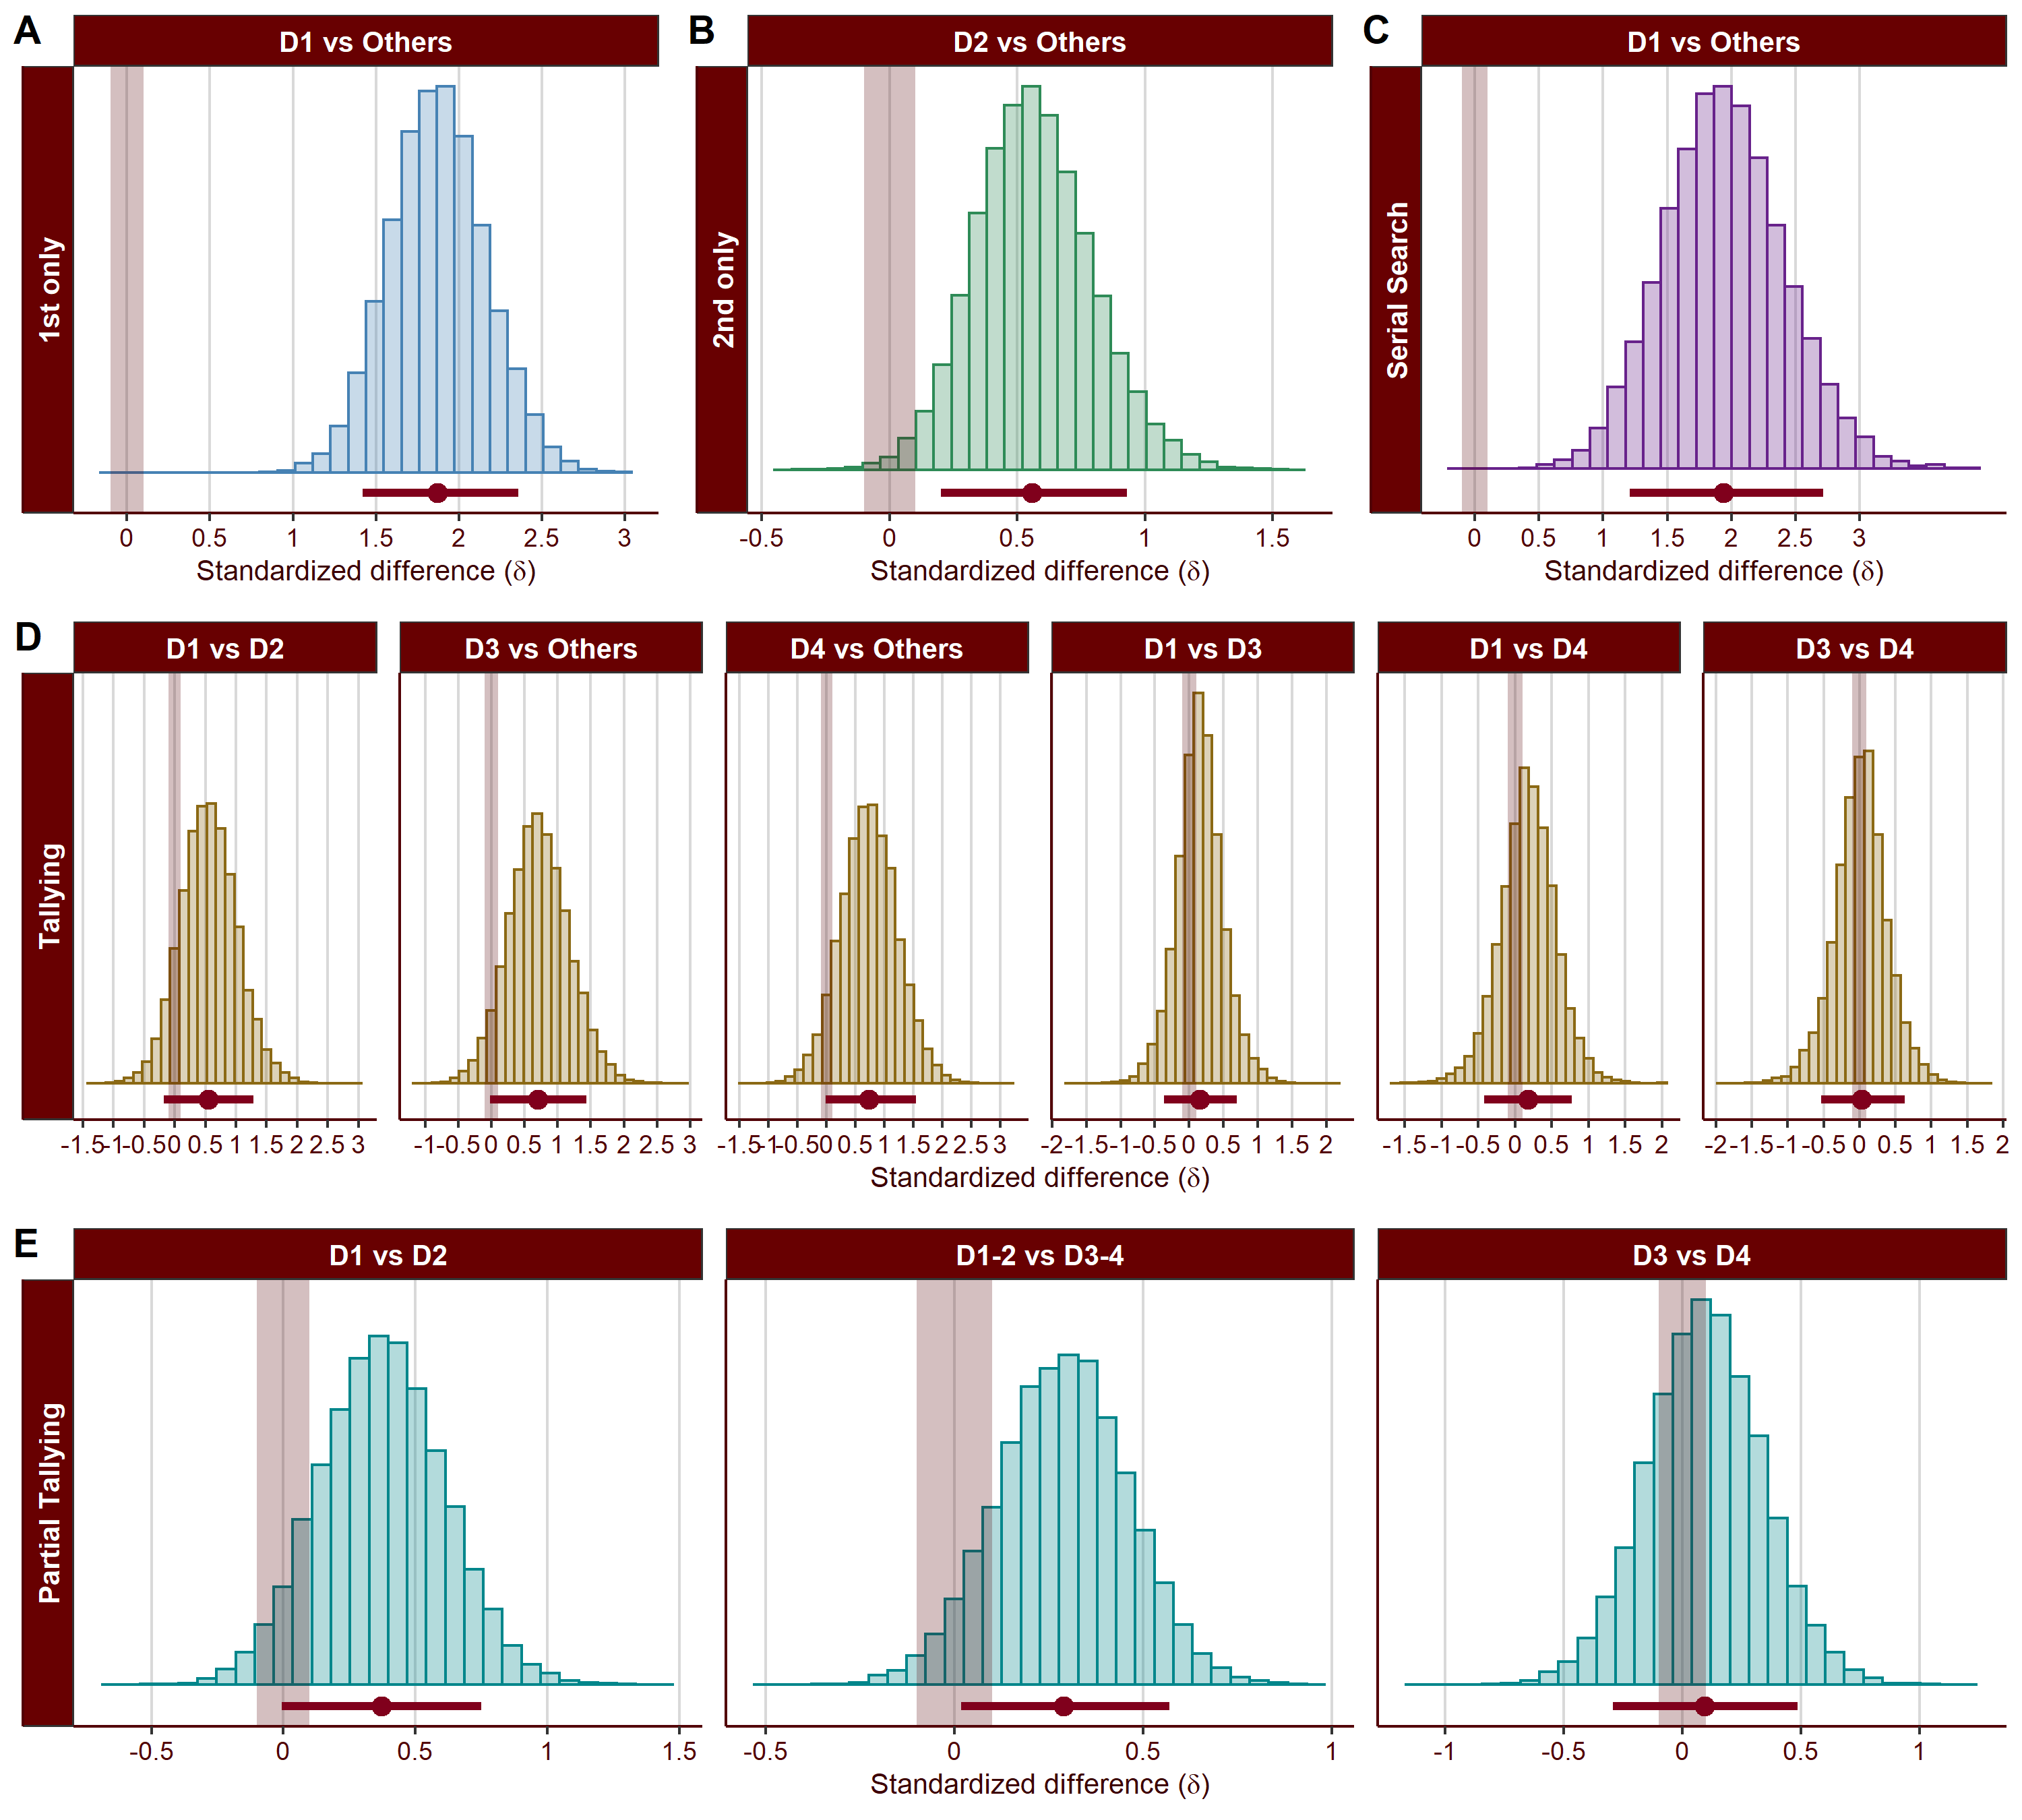
\includegraphics{C:/Users/rerr_/Google Drive/Graduate/Lab/Studies/MultiCue_Probabilistic/Stages/Shifted Weights/Eye Tracking/Analysis/Figures/SC1_first_comparisons.png}
\caption{(\#fig:first-comparisons)Follow up comparisons for the
allocation of first fixations, across decision groups. The horizontal
red bar represents the 0.89 HDI. The shaded area highlights the ROPE
used in these comparisons}
\end{figure}

\begin{figure}
\centering
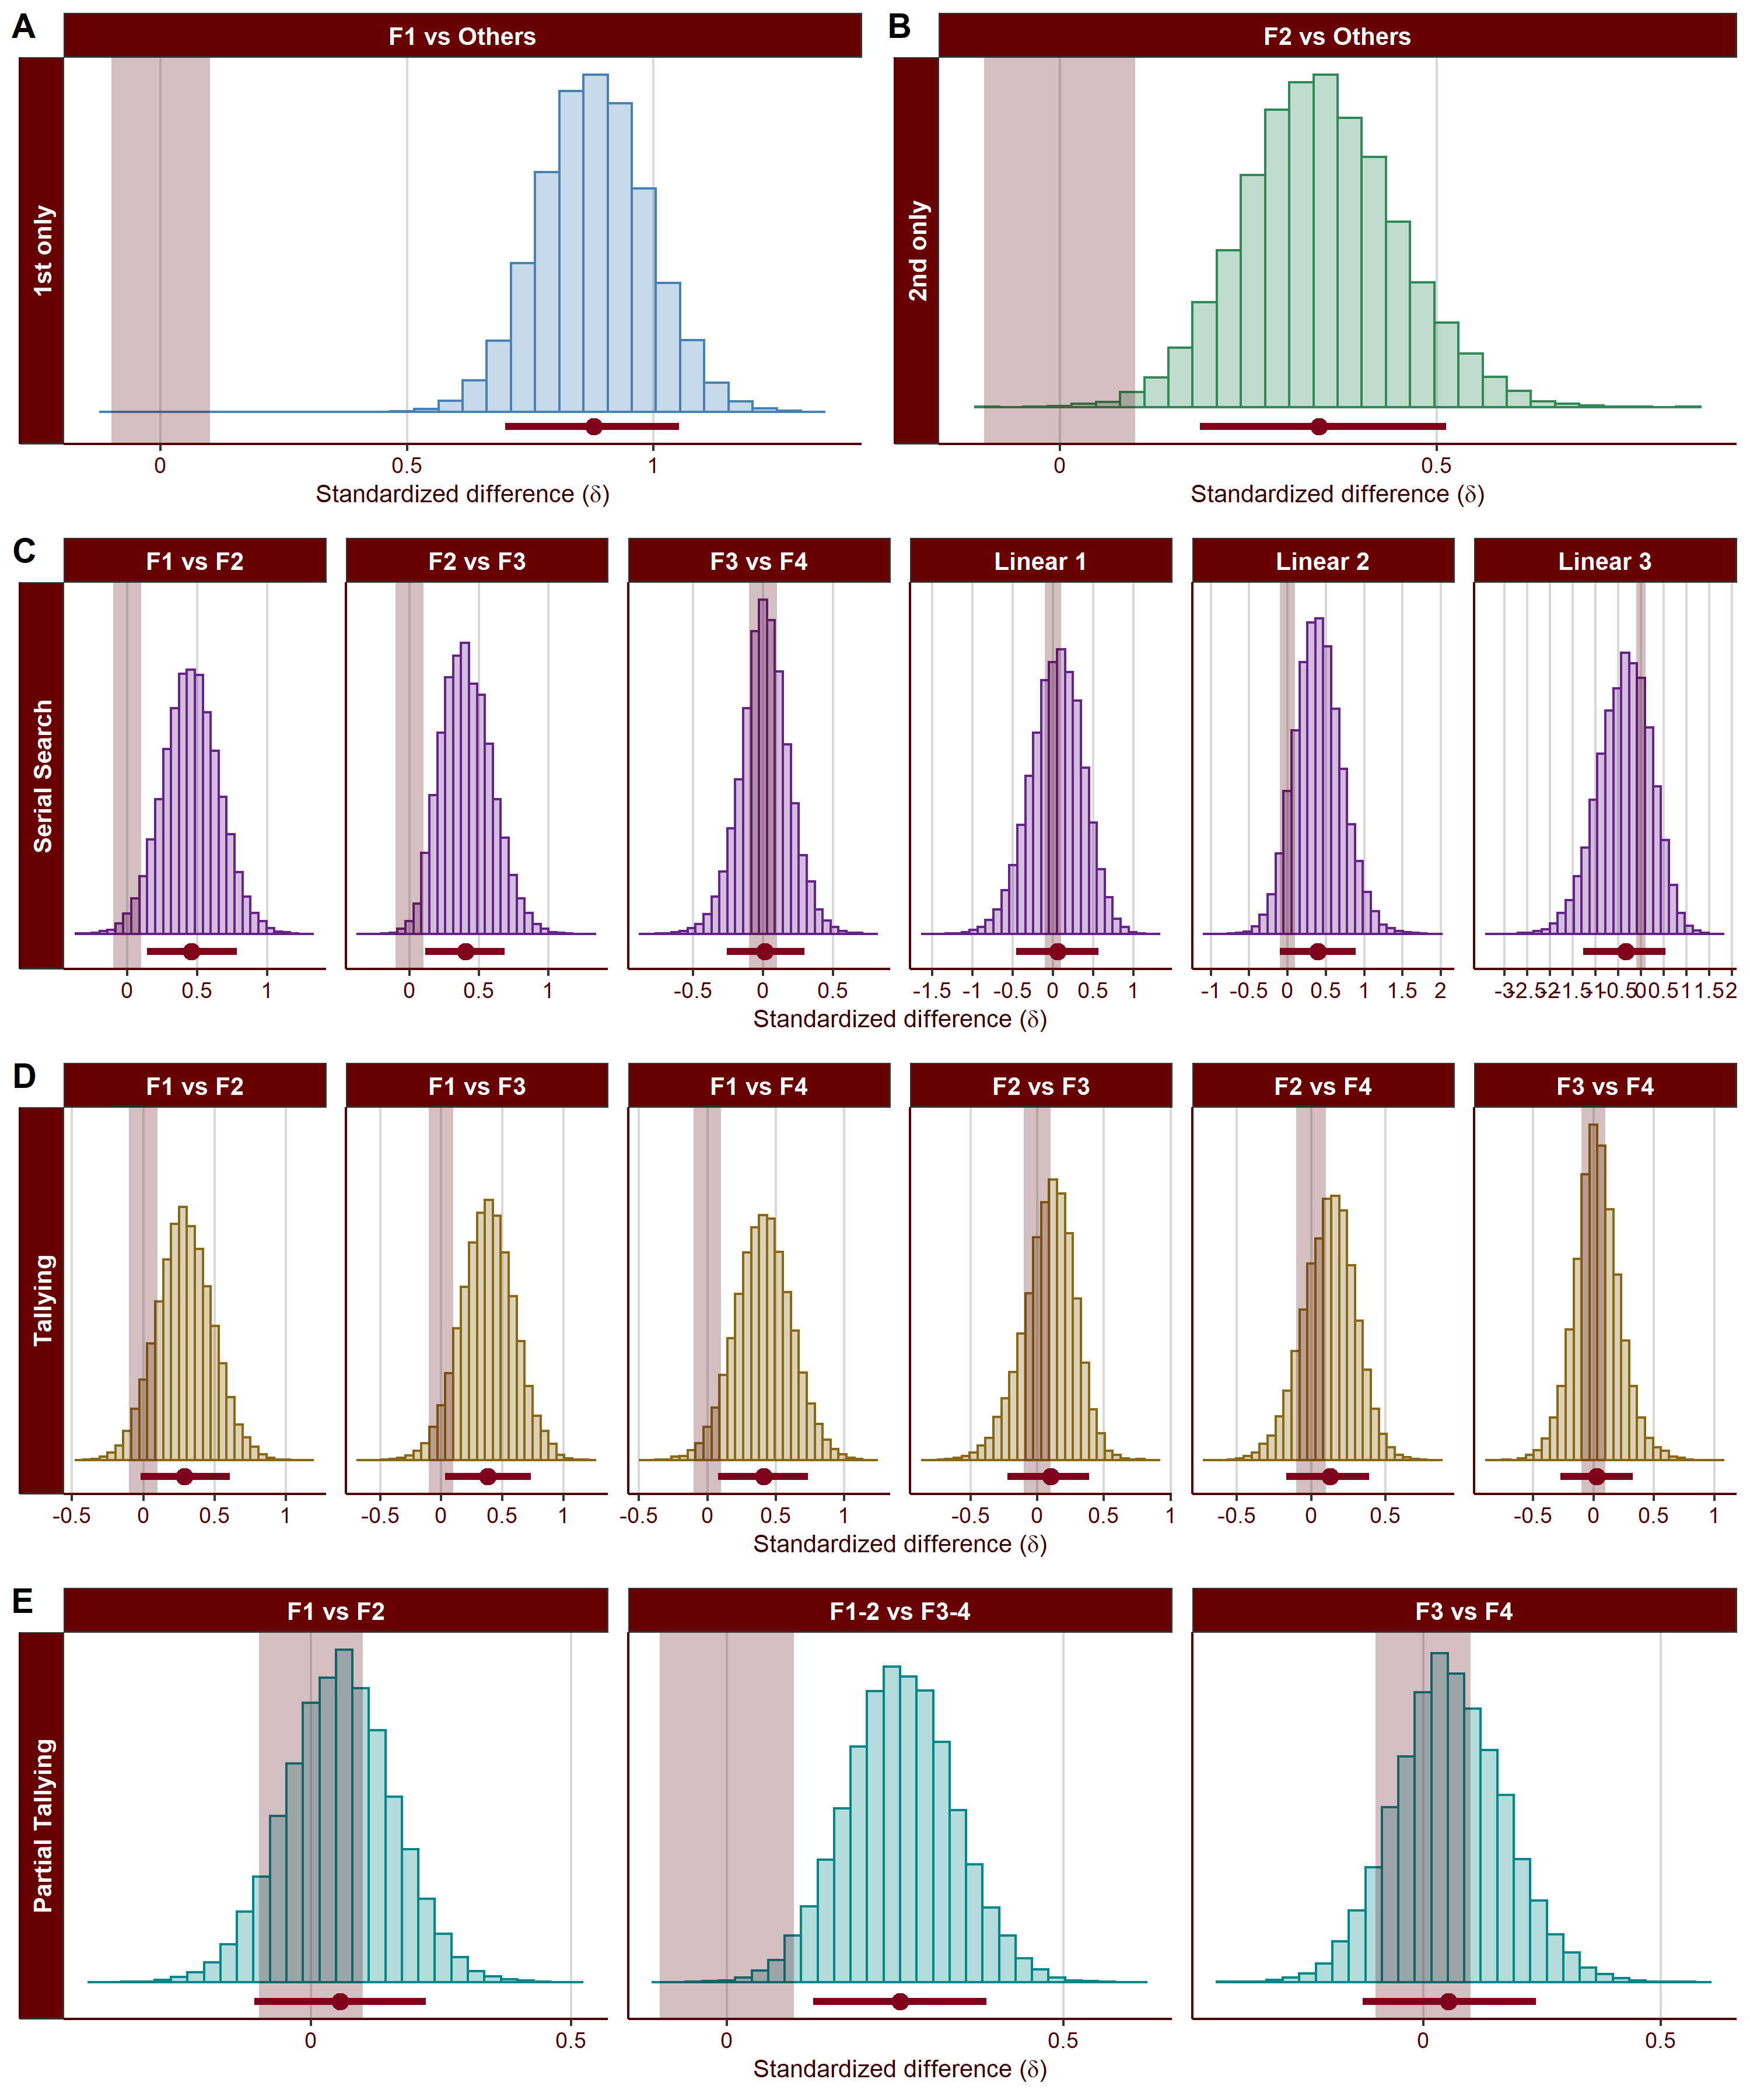
\includegraphics{C:/Users/rerr_/Google Drive/Graduate/Lab/Studies/MultiCue_Probabilistic/Stages/Shifted Weights/Eye Tracking/Analysis/Figures/SD1_proportion_comparisons.png}
\caption{(\#fig:proportion-comparisons)Follow up comparisons for the
allocation of fixations. The horizontal red bar represents the 0.89 HDI.
The shaded area highlights the ROPE used in these comparisons}
\end{figure}

\begin{figure}
\centering
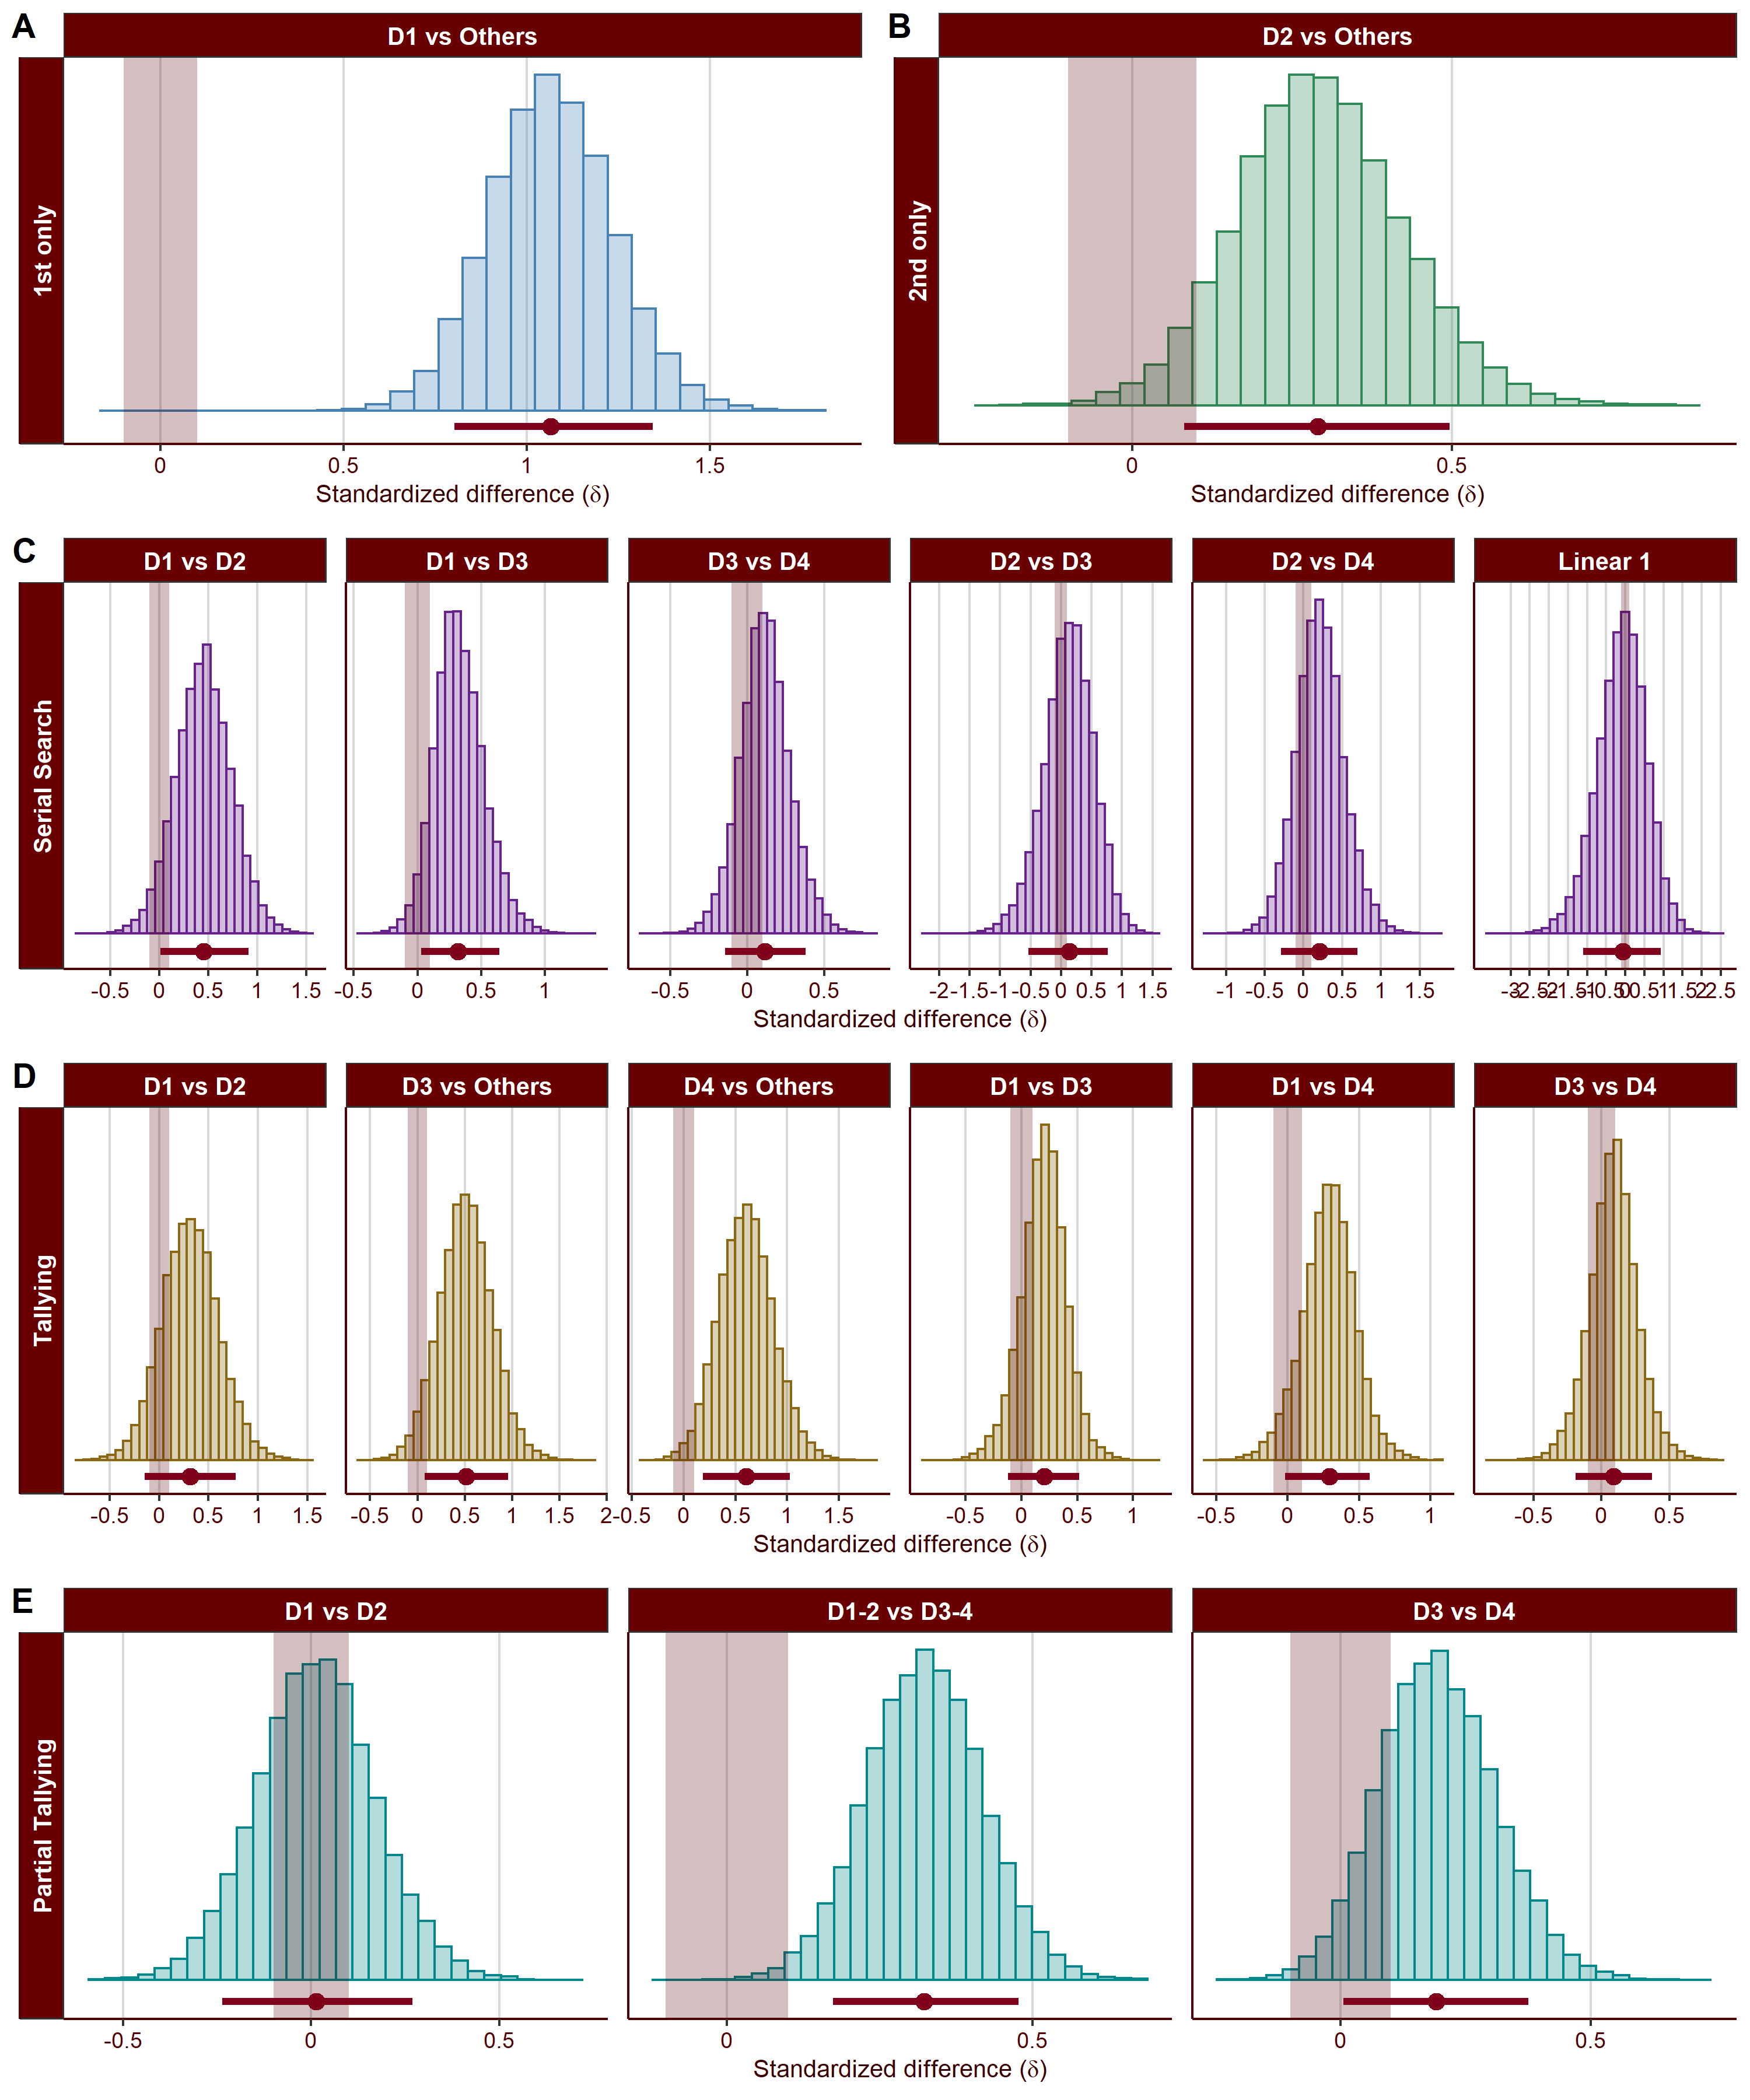
\includegraphics{C:/Users/rerr_/Google Drive/Graduate/Lab/Studies/MultiCue_Probabilistic/Stages/Shifted Weights/Eye Tracking/Analysis/Figures/SE1_last_comparisons.png}
\caption{(\#fig:last-comparisons)Follow up comparisons for the
allocation of last fixations. The horizontal red bar represents the 0.89
HDI. The shaded area highlights the ROPE used in these comparisons}
\end{figure}

\begin{figure}[!b]
    \centering
    \begin{subfigure}{1\textwidth}
        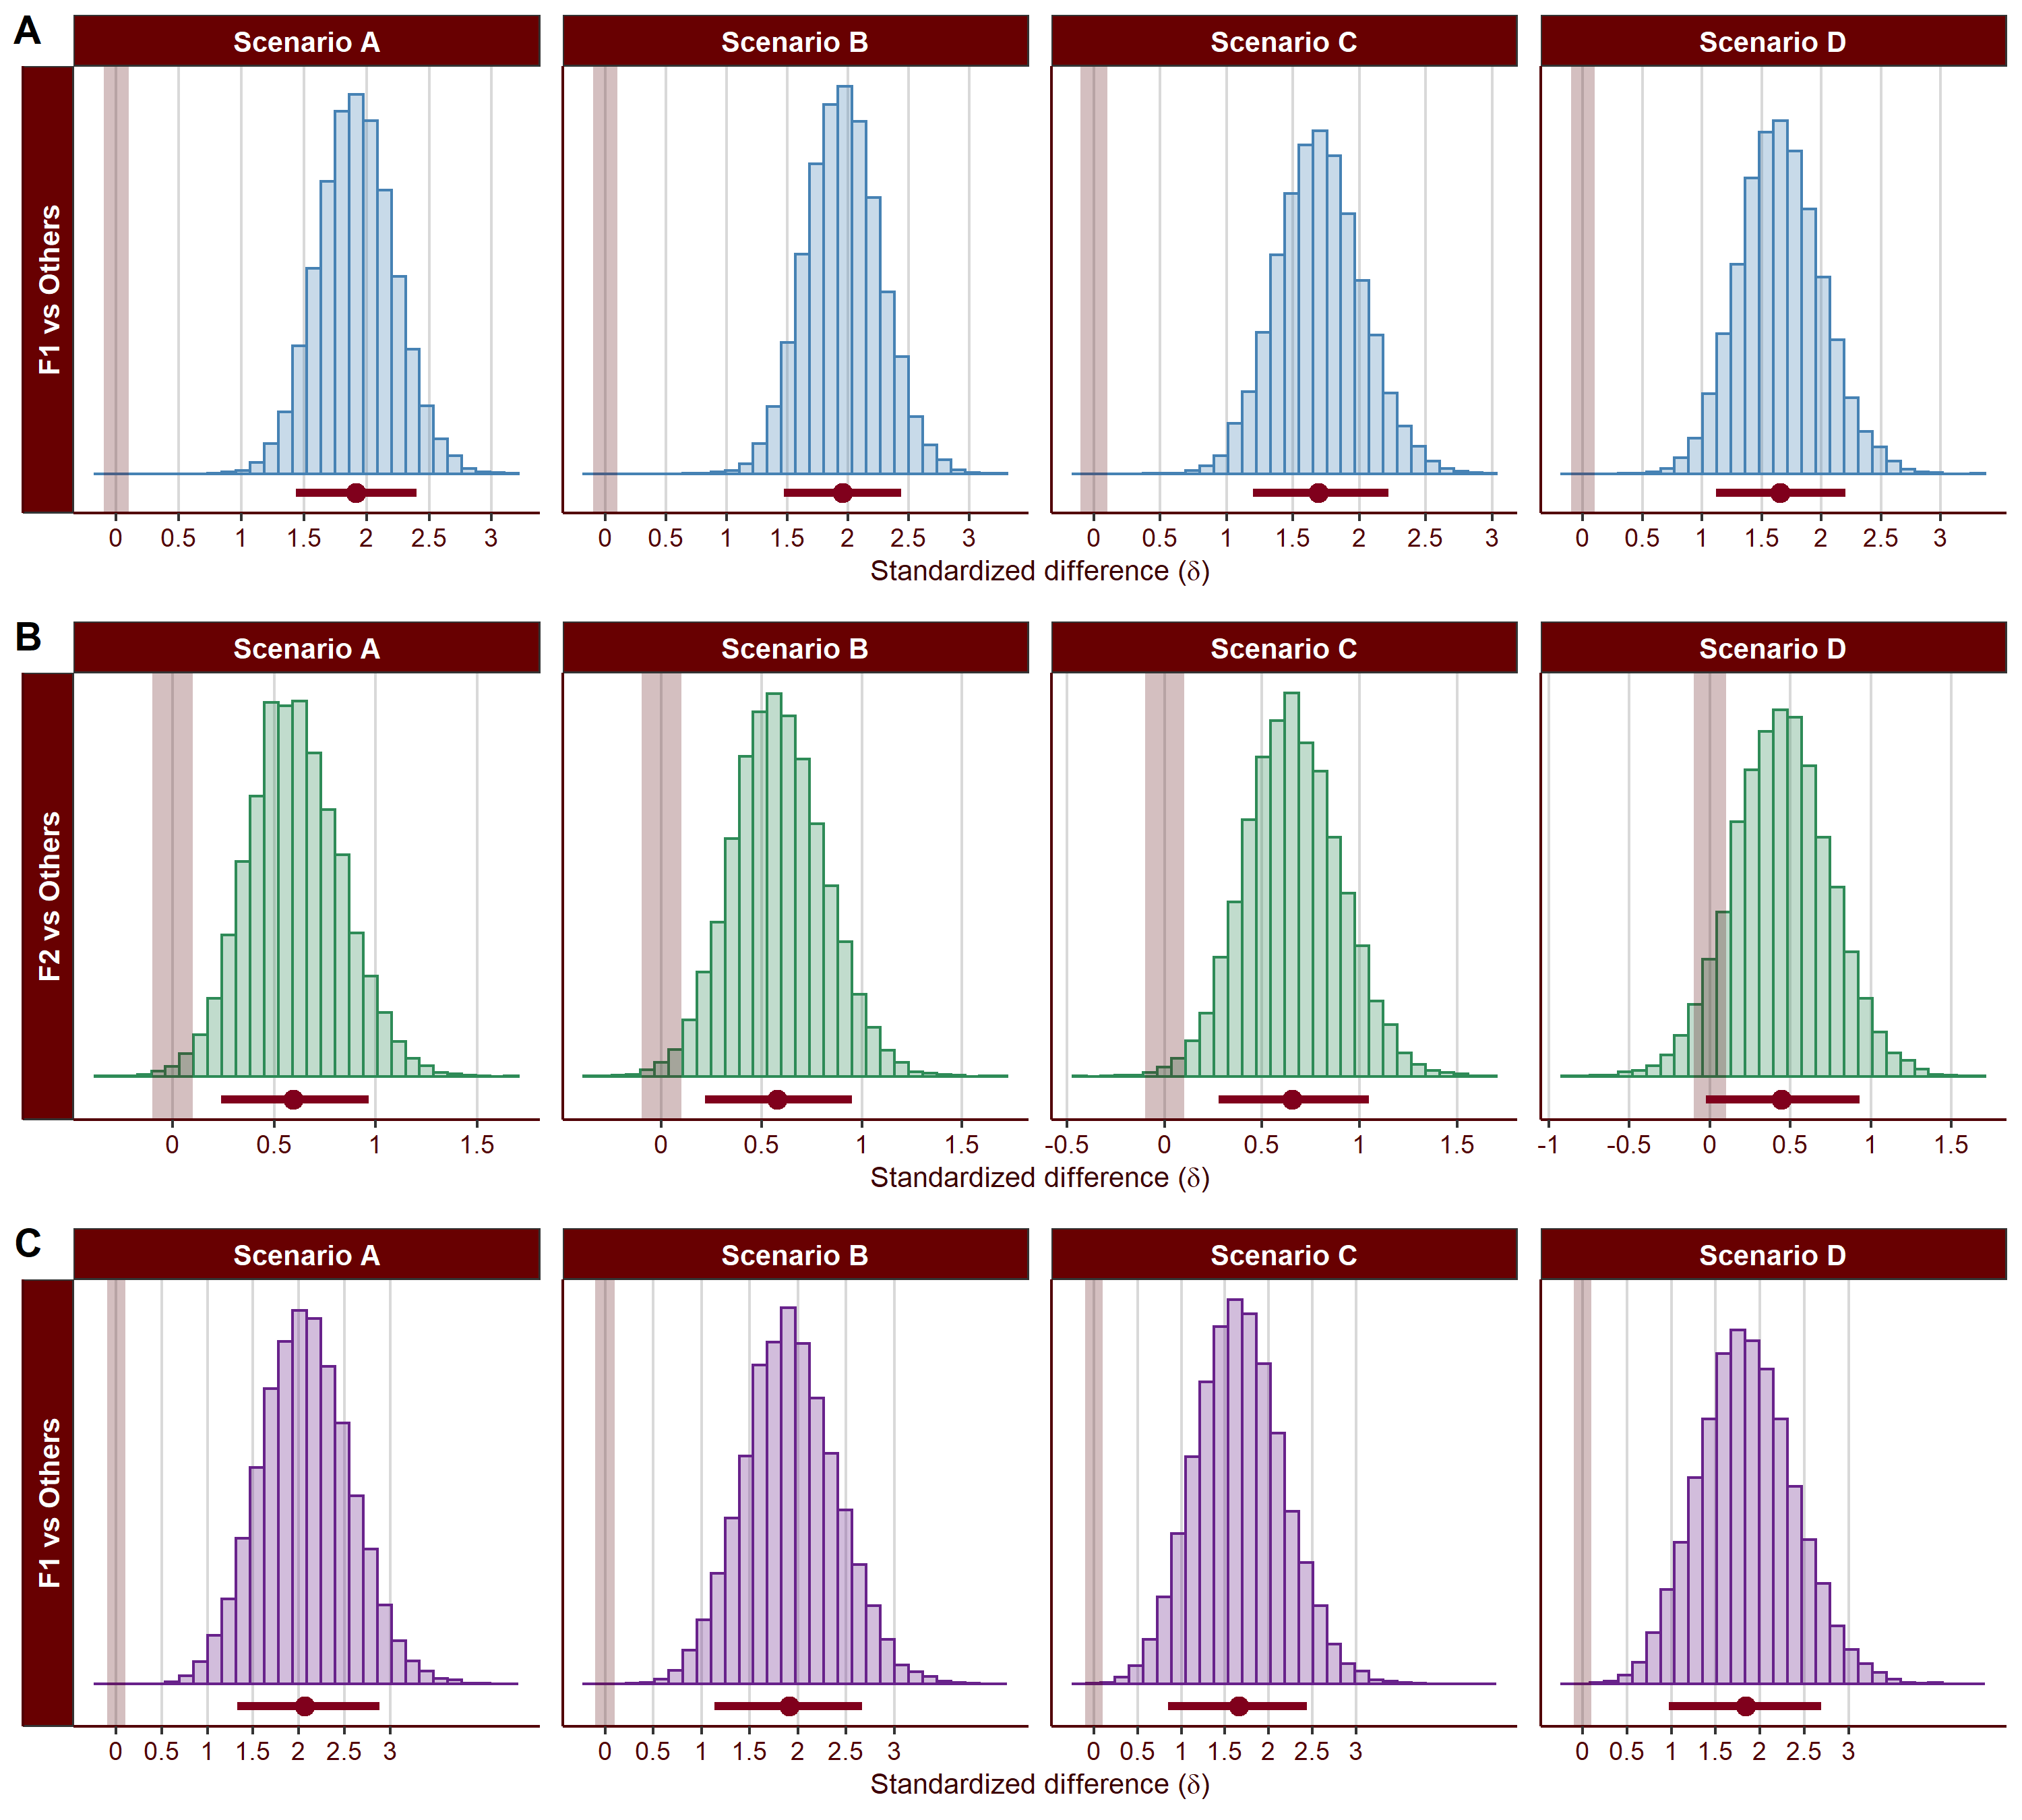
\includegraphics[width=\linewidth]{Figures/SC2_first_scenario_comparisons_A.png}
        \subcaption{1st only (A), 2nd only (B), Serial search (C)}
        \label{fig:first-scenario-comparisons-A}
    \end{subfigure}
    \caption[]{Follow up comparisons for the allocation of first fixations across decision groups in the different decision scenarios. The horizontal red bar represents the 0.89 HDI. The shaded area highlights the ROPE used in these comparisons}
\end{figure}

\medskip

\begin{figure}[ht]\ContinuedFloat
    \centering
    \begin{subfigure}{1\textwidth}
        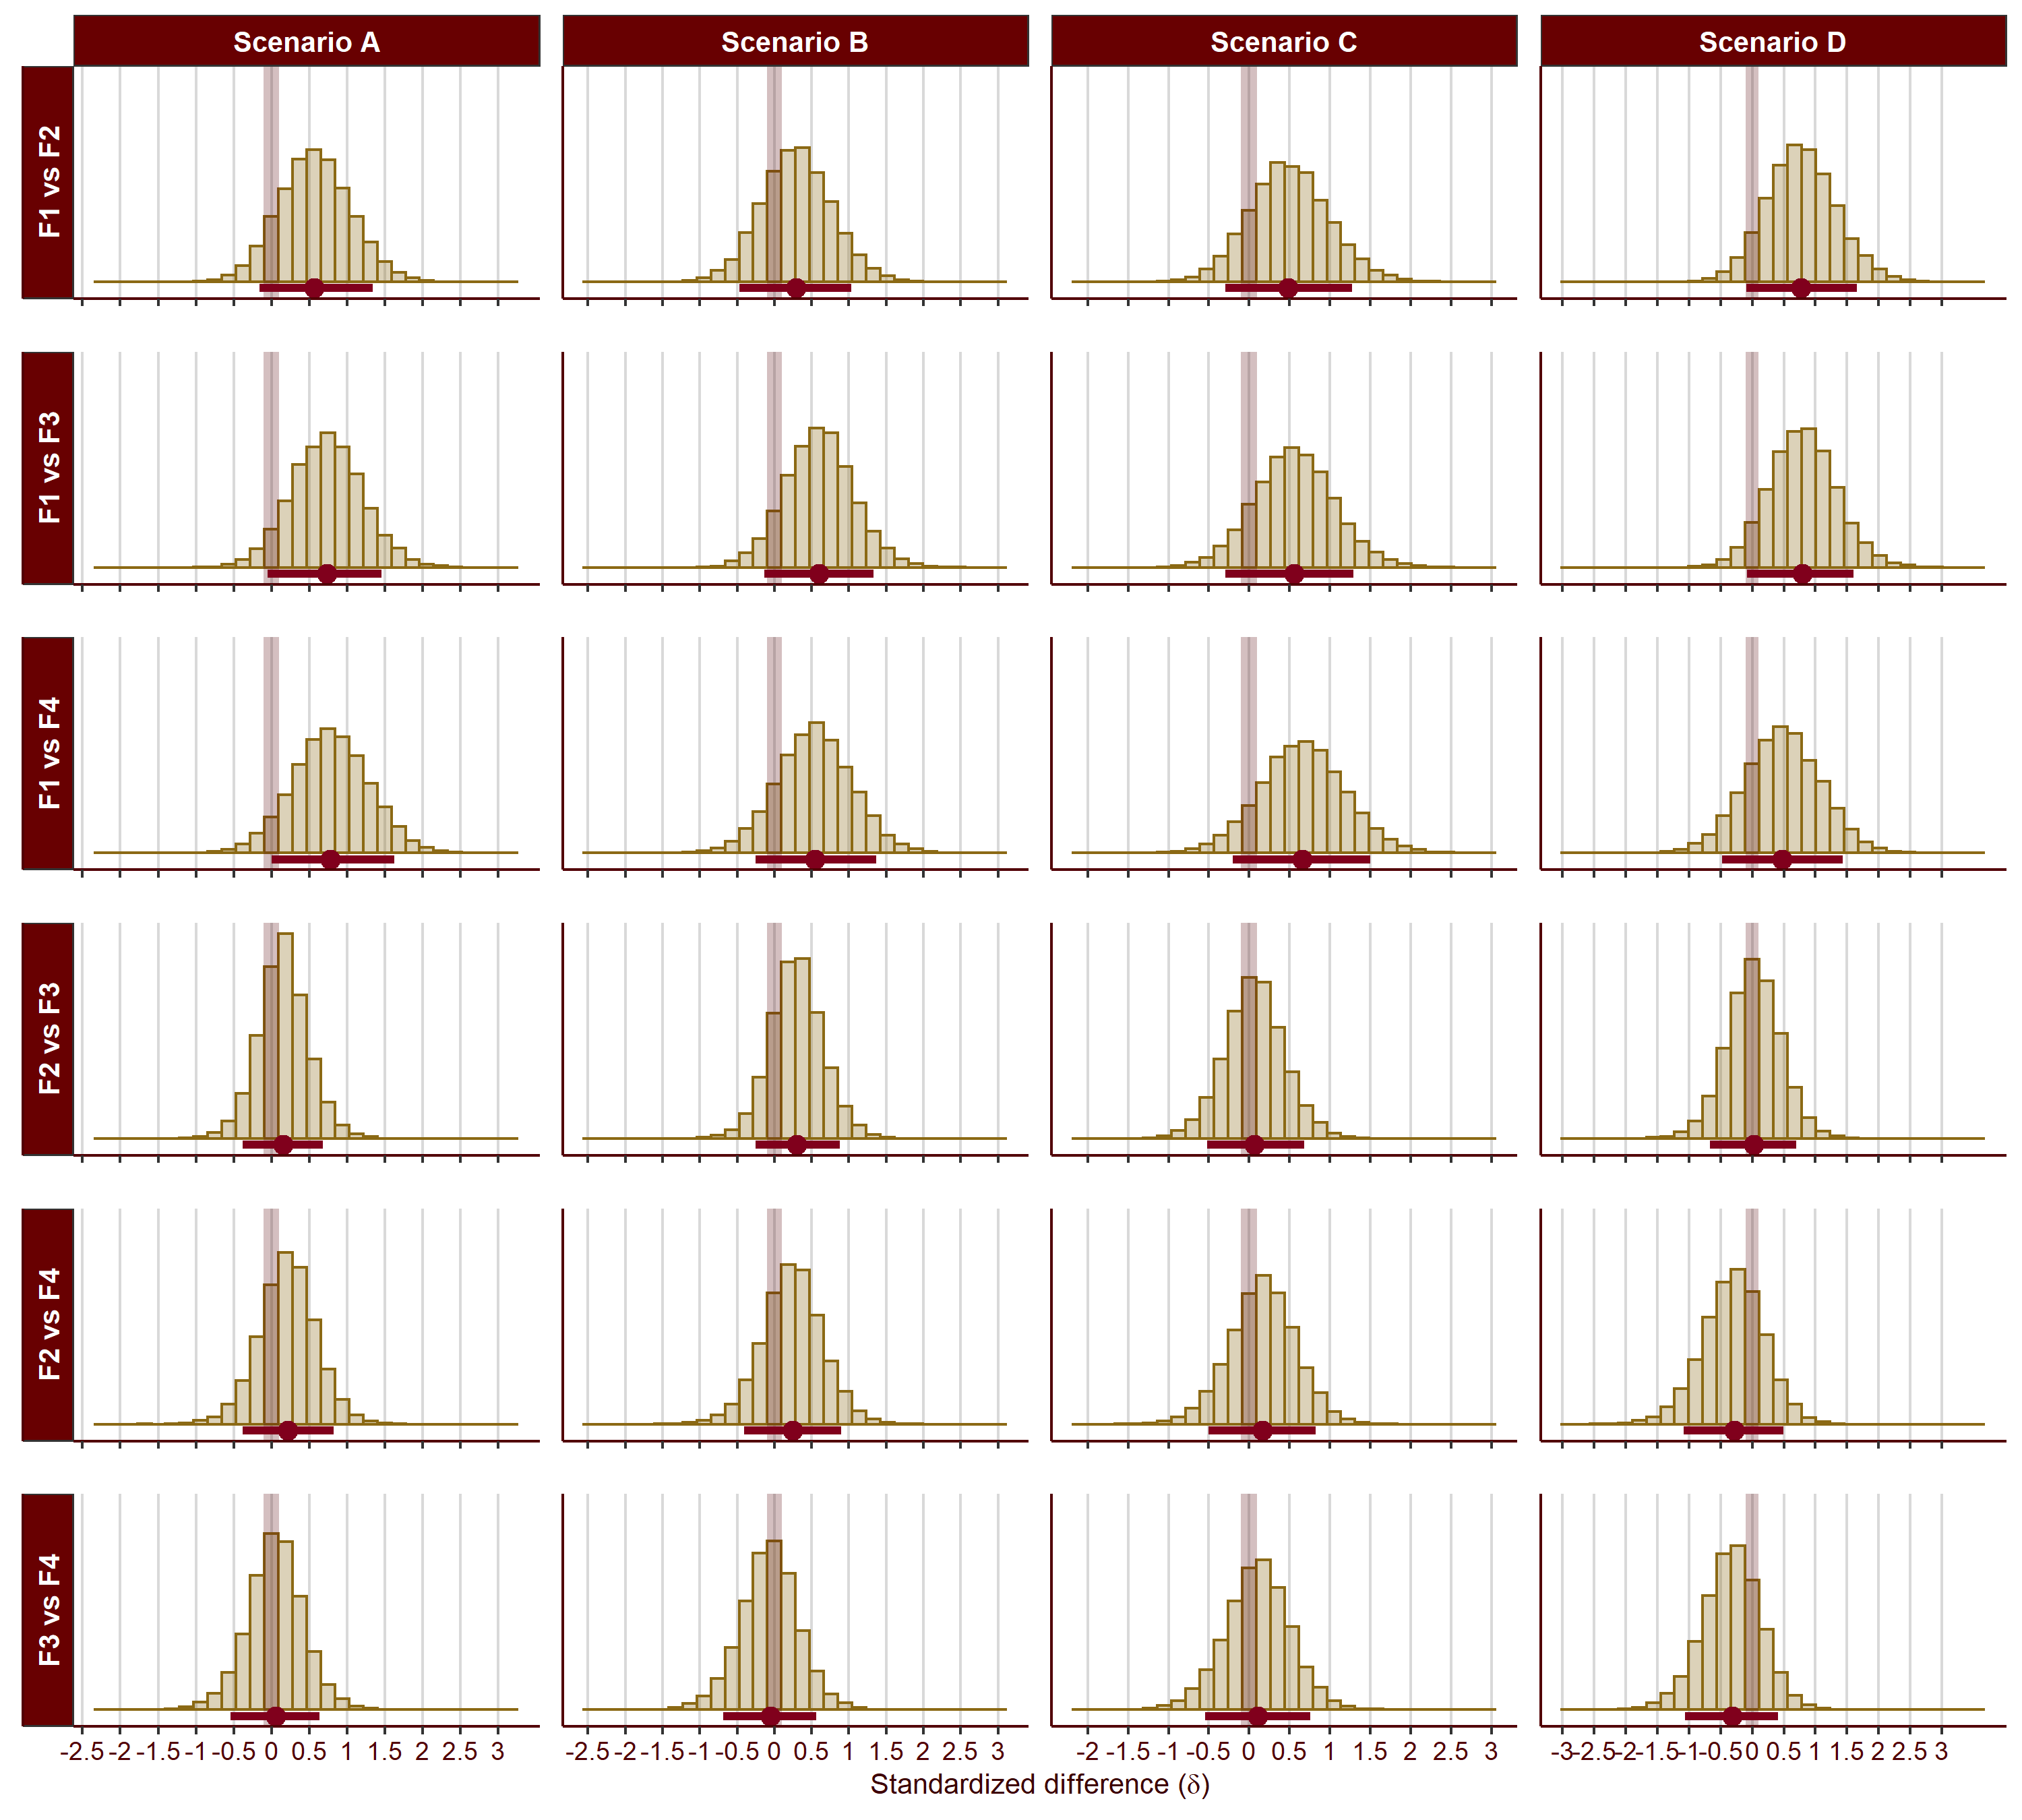
\includegraphics[width=\linewidth]{Figures/SC2_first_scenario_comparisons_B.png}
        \subcaption{Tallying}
        \label{fig:first-scenario-comparisons-B}
    \end{subfigure}
    \caption[]{Continued}
\end{figure}

\medskip

\begin{figure}[ht]\ContinuedFloat
    \centering
    \begin{subfigure}{1\textwidth}
        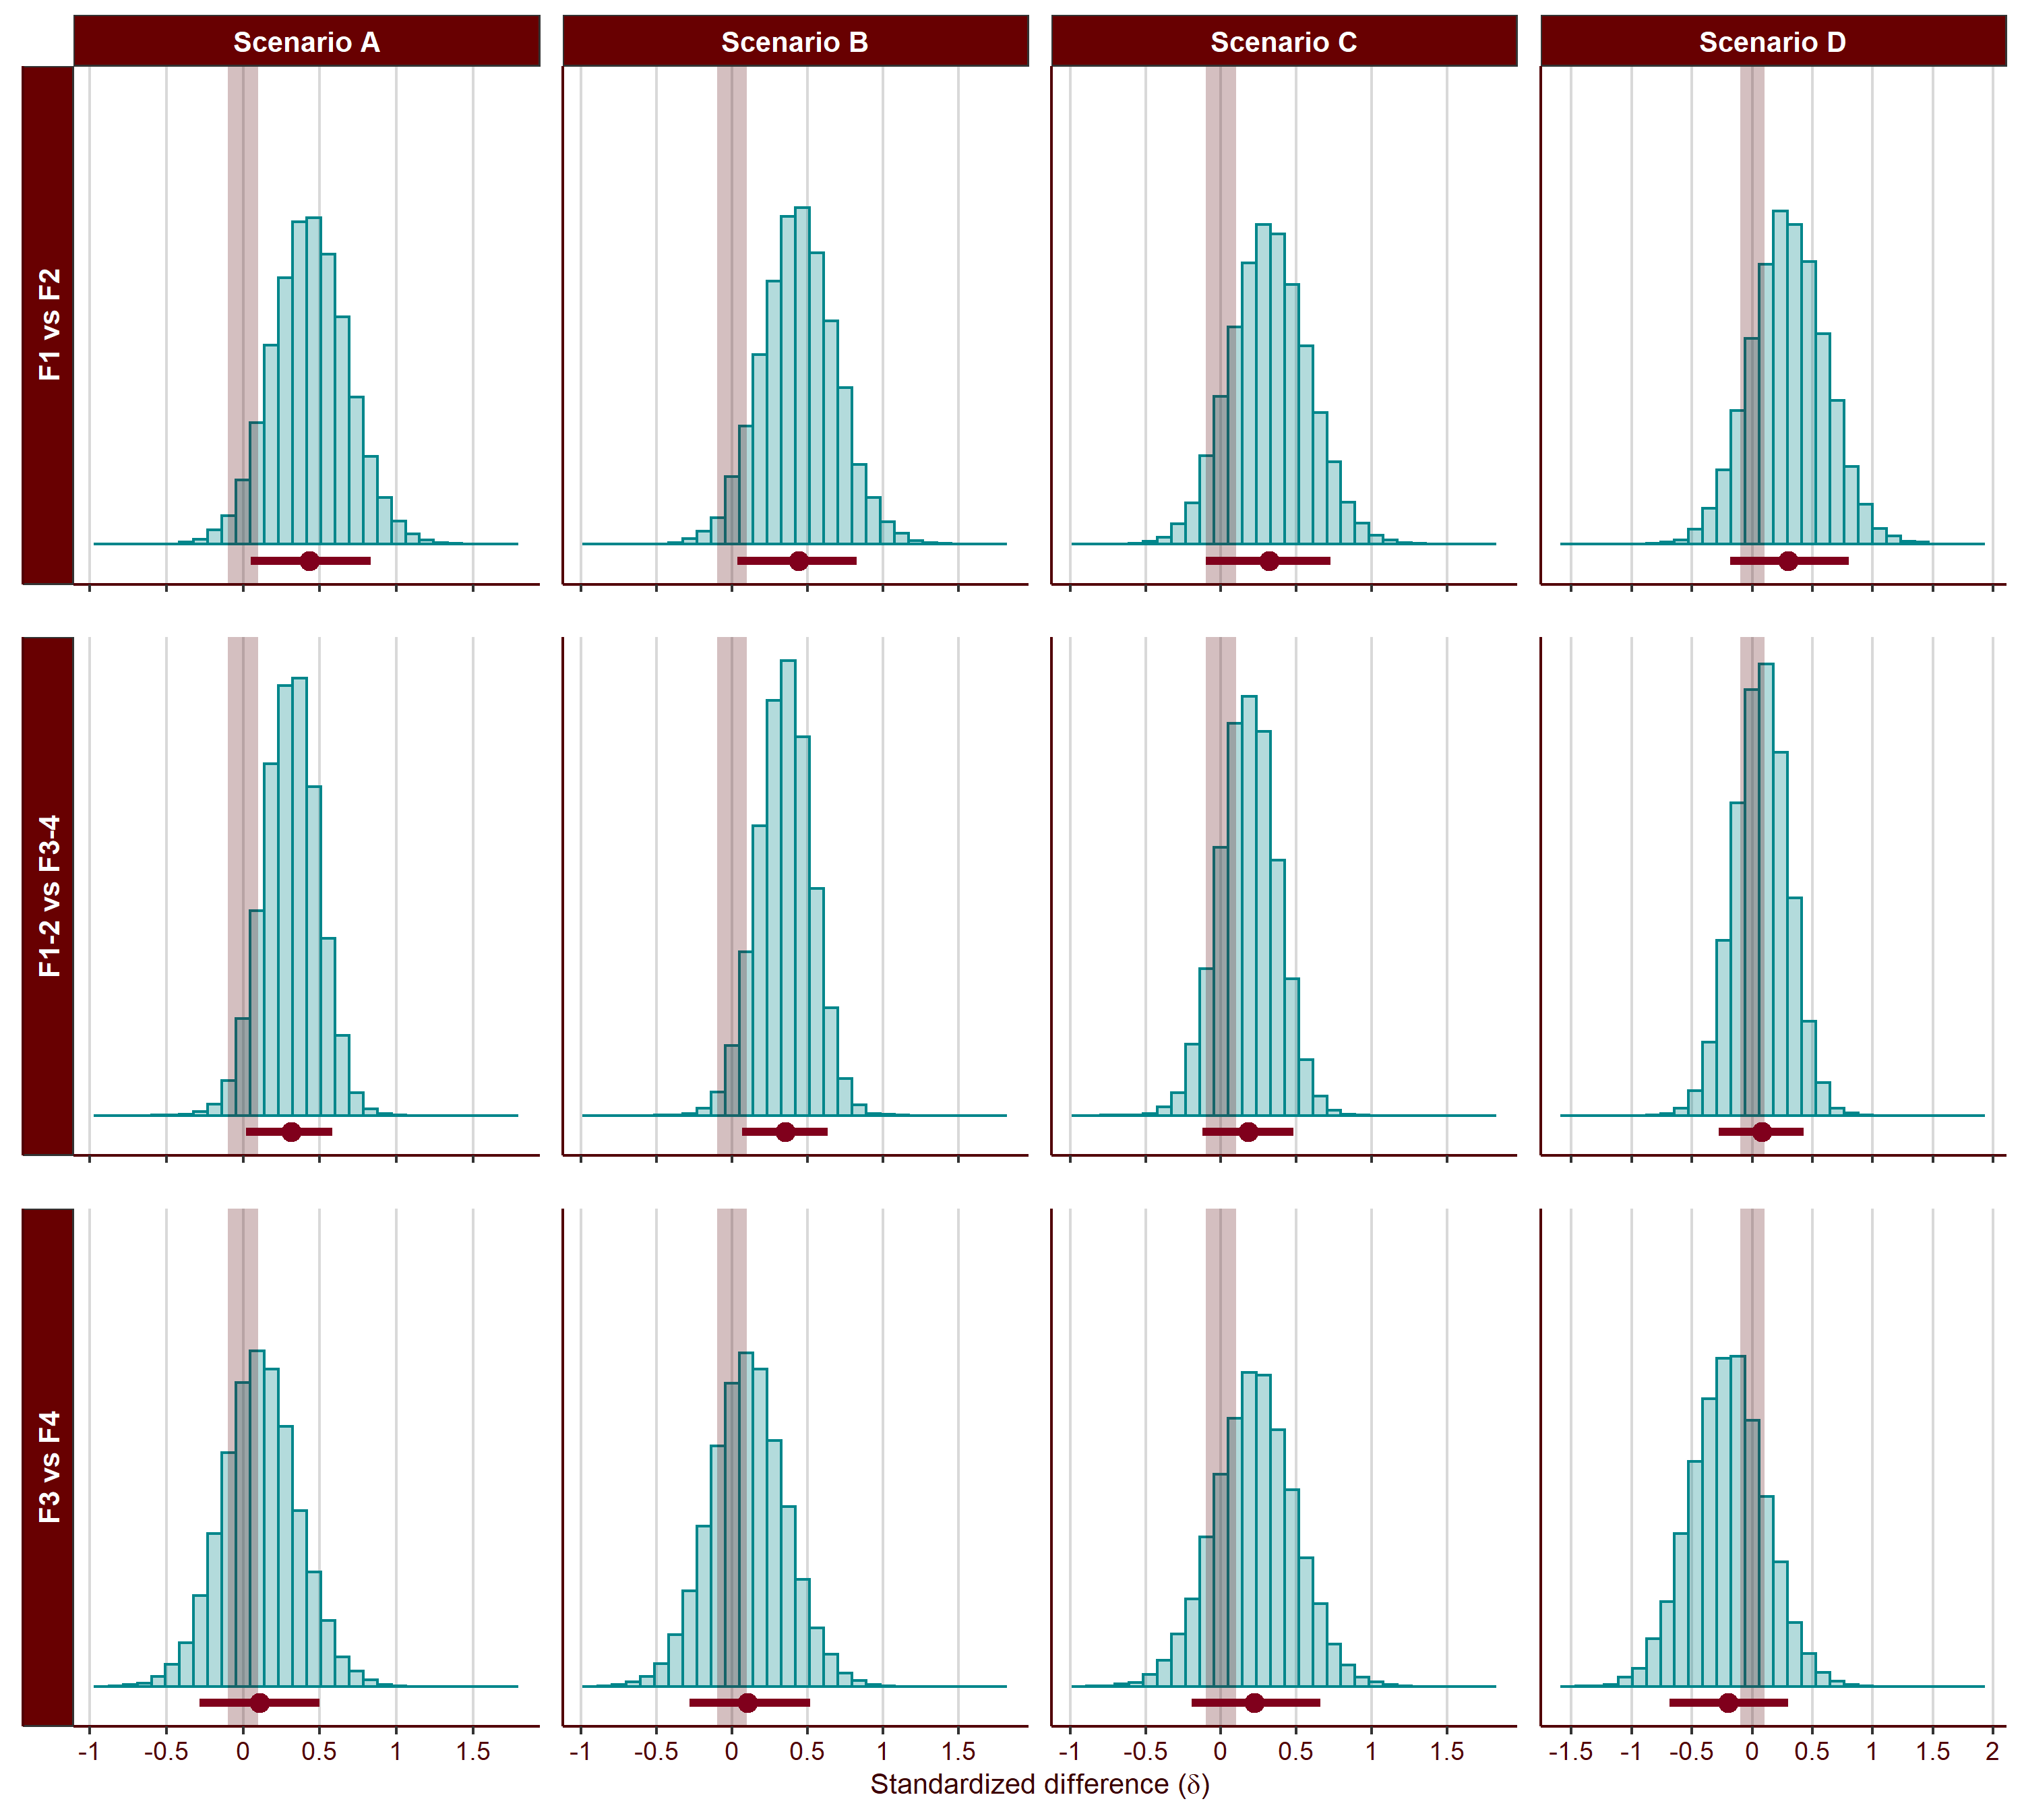
\includegraphics[width=\linewidth]{Figures/SC2_first_scenario_comparisons_C.png}
        \subcaption{Partial Tallying}
        \label{fig:first-scenario-comparisons-C}
    \end{subfigure}
    \caption[]{Continued}
    \label{fig:first-scenario-comparisons}
\end{figure}

\begin{figure}[!b]
    \centering
    \begin{subfigure}{1\textwidth}
        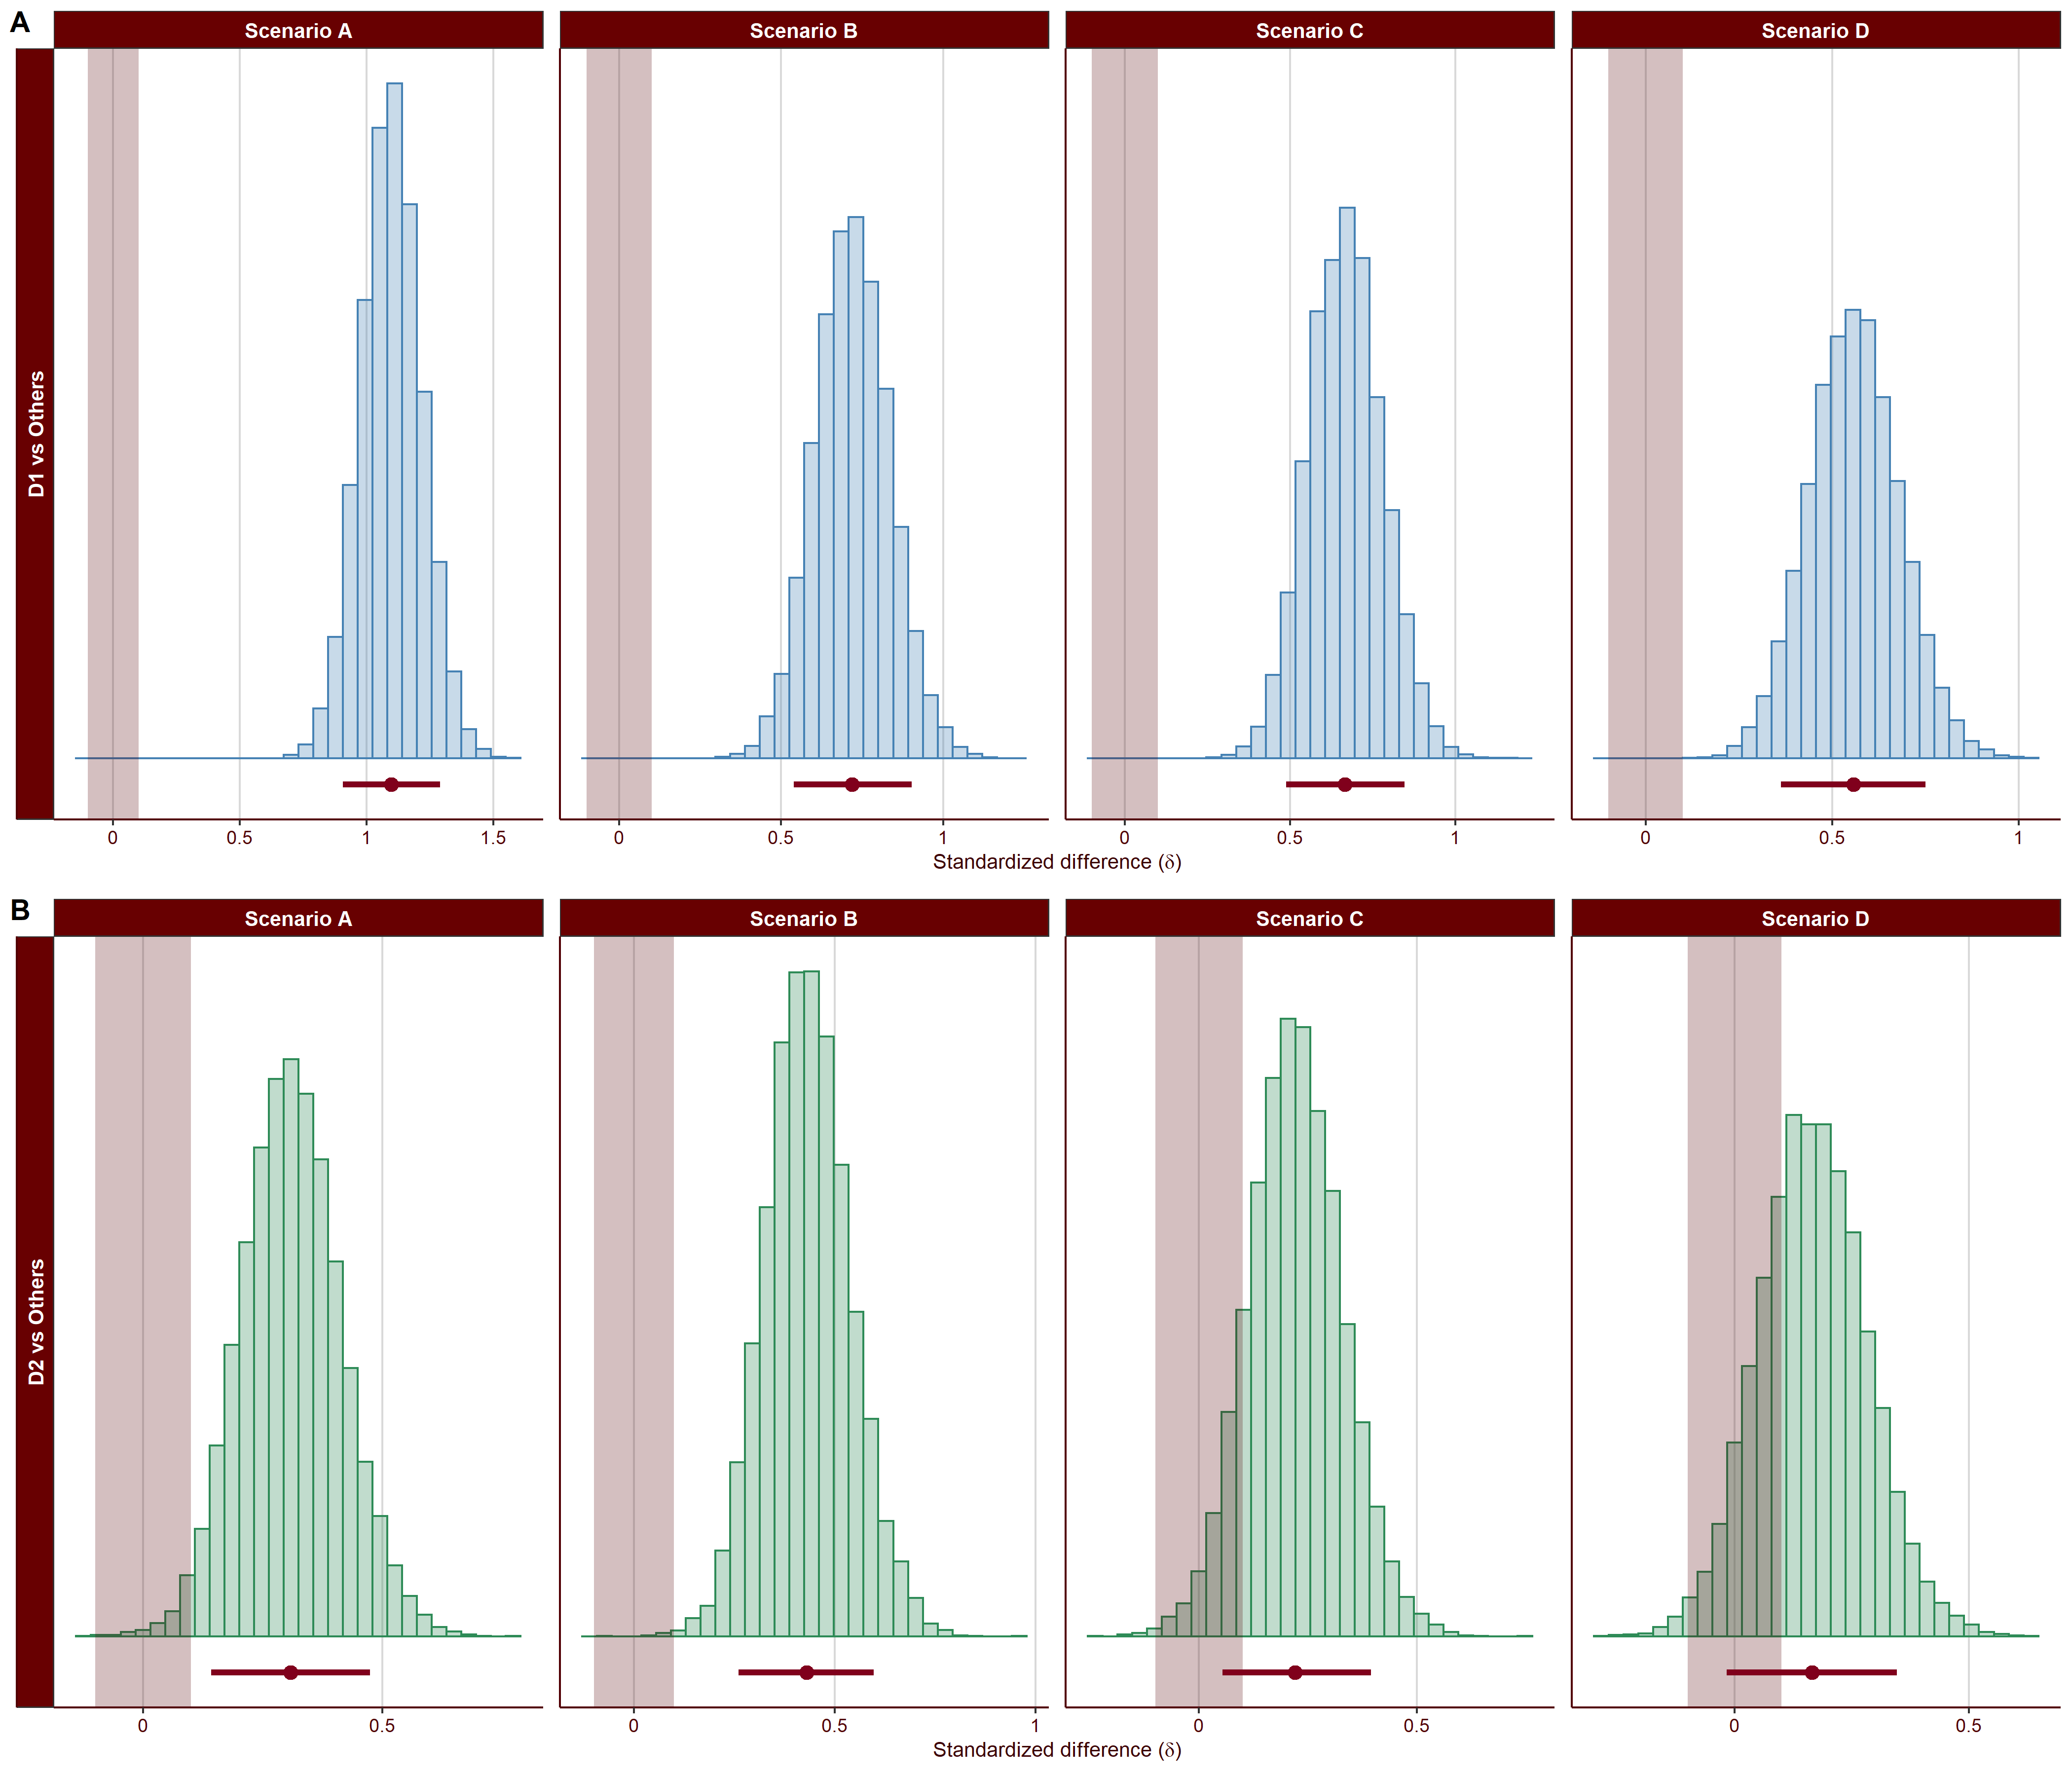
\includegraphics[width=\linewidth]{Figures/SD2_proportion_scenario_comparisons_A.png}
        \subcaption{1st only (A), 2nd only (B)}
        \label{fig:proportion-scenario-comparisons-A}
    \end{subfigure}
    \caption[]{Follow up comparisons for the allocation of fixations across decision groups in the different decision scenarios. The horizontal red bar represents the 0.89 HDI. The shaded area highlights the ROPE used in these comparisons}
\end{figure}

\medskip

\begin{figure}[ht]\ContinuedFloat
    \centering
    \begin{subfigure}{1\textwidth}
        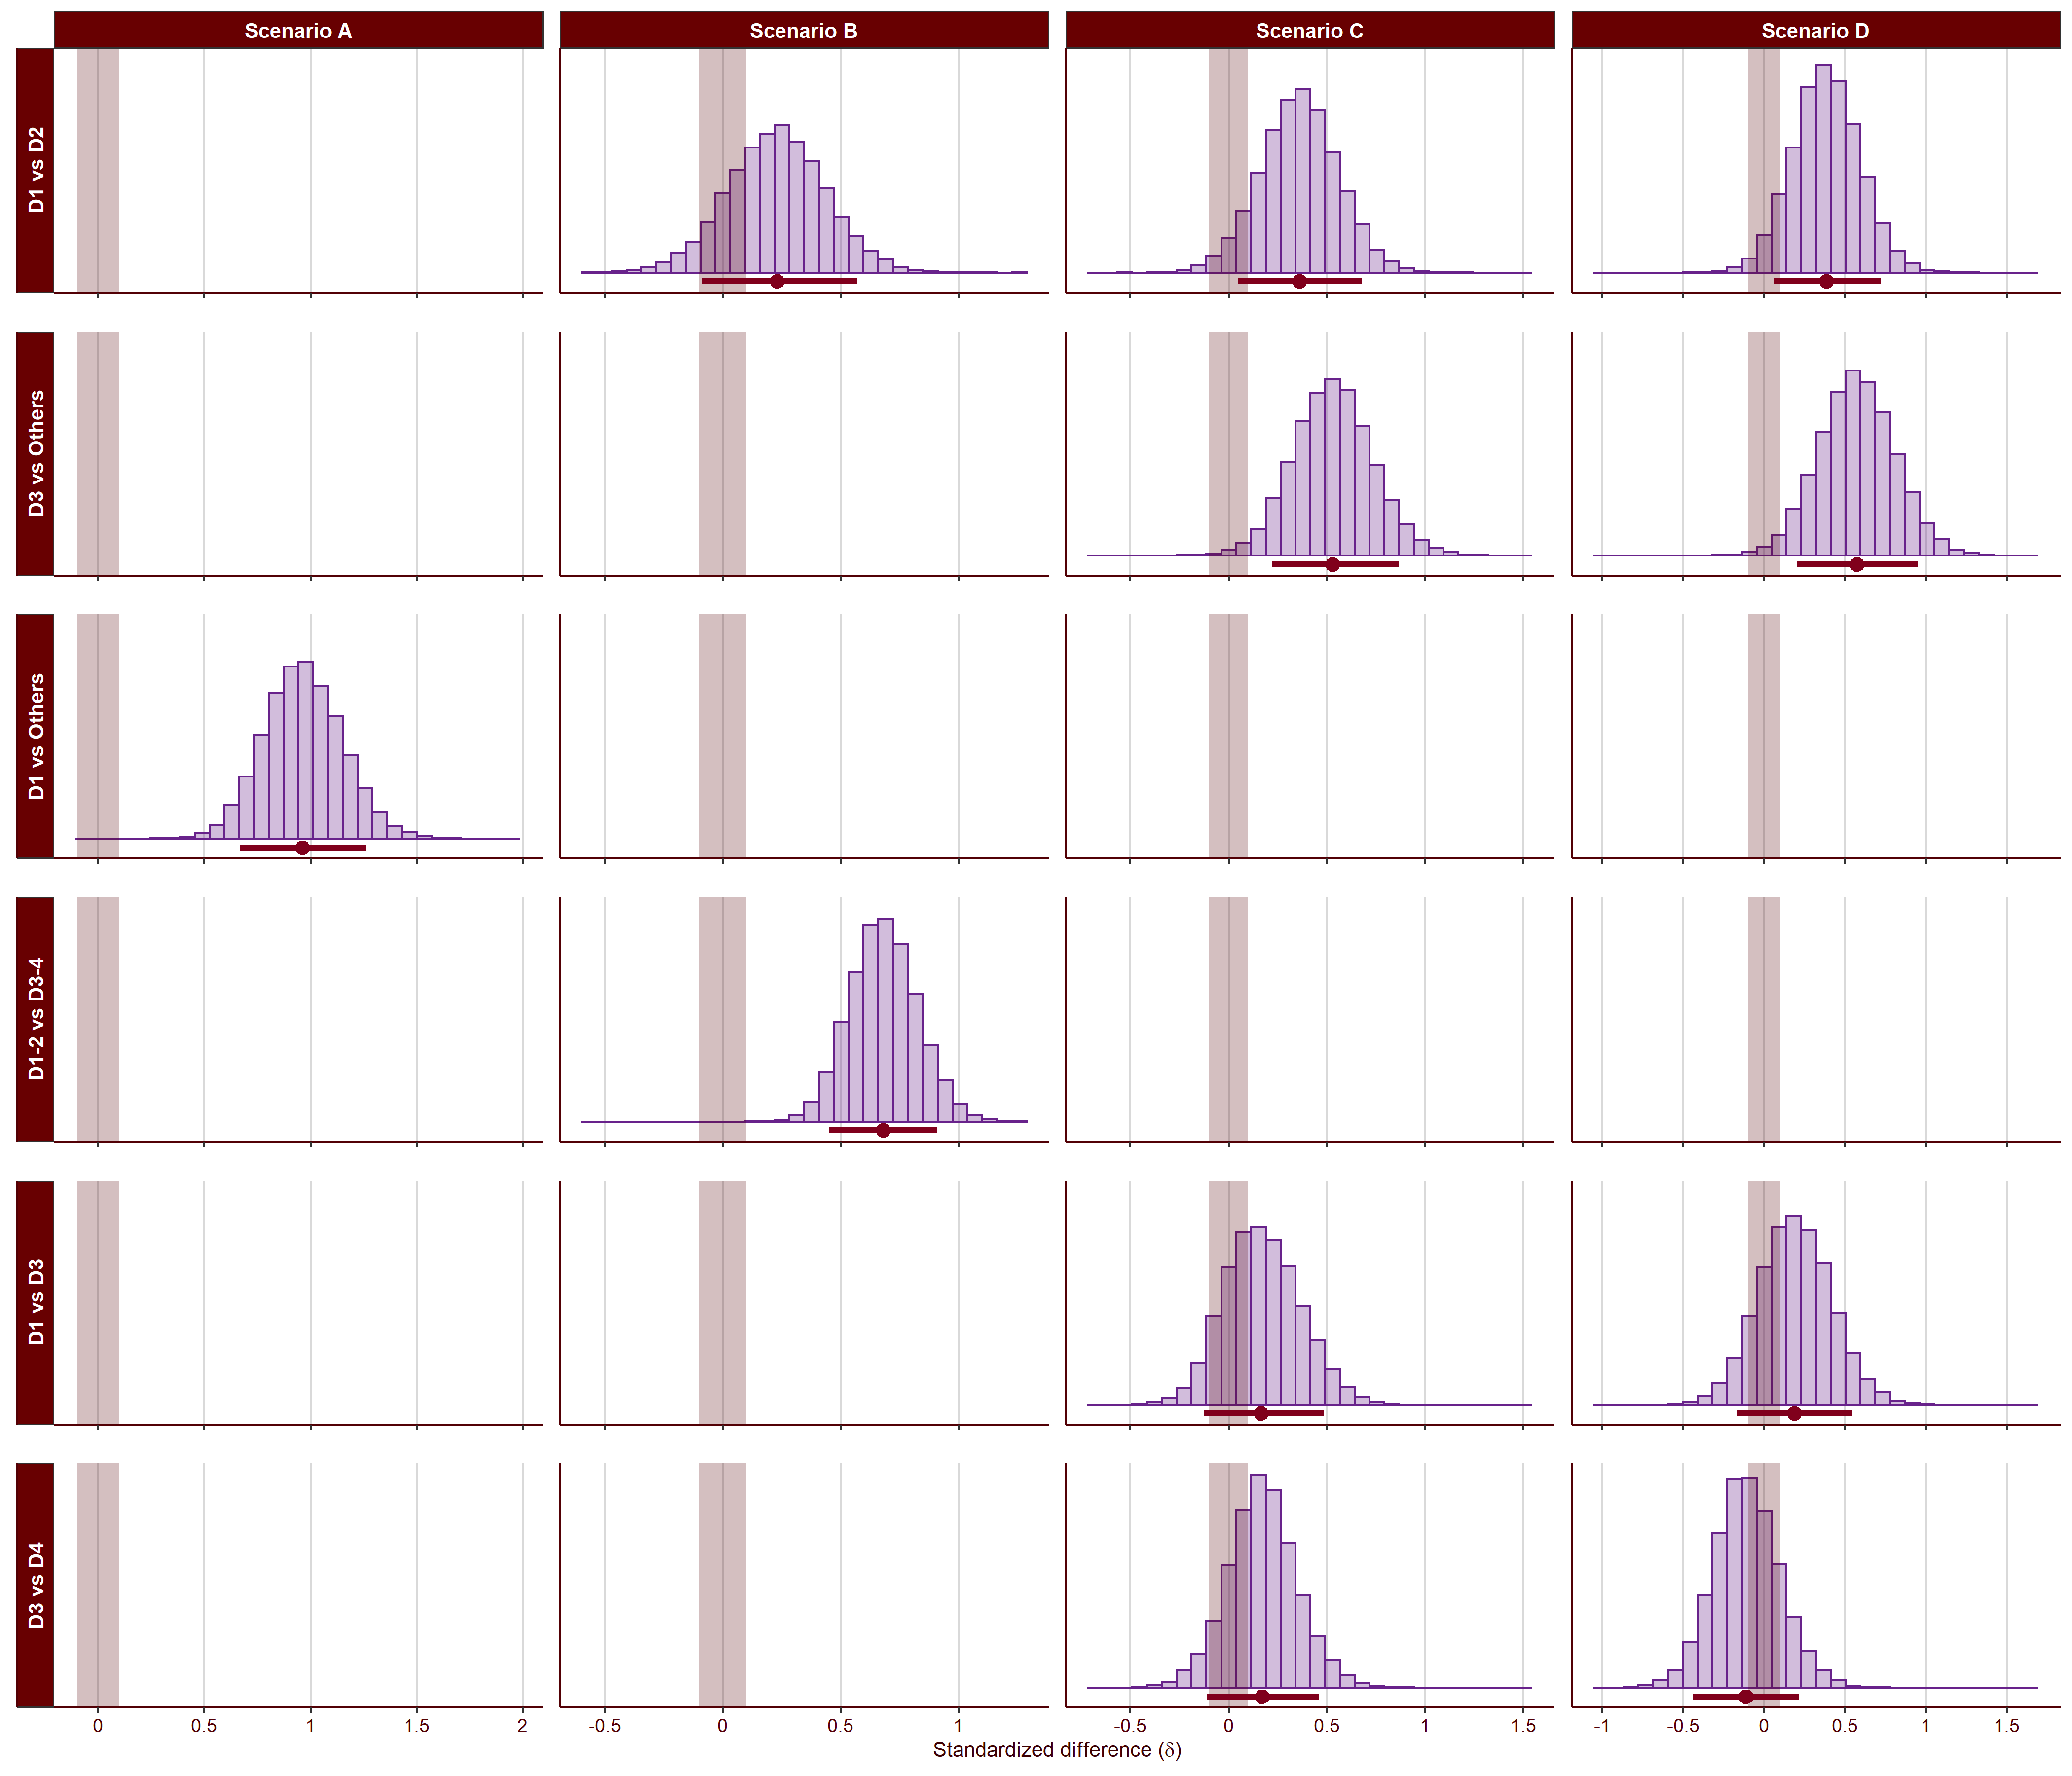
\includegraphics[width=\linewidth]{Figures/SD2_proportion_scenario_comparisons_B.png}
        \subcaption{Serial Search}
        \label{fig:proportion-scenario-comparisons-B}
    \end{subfigure}
    \caption[]{Continued}
\end{figure}

\medskip

\begin{figure}[ht]\ContinuedFloat
    \centering
    \begin{subfigure}{1\textwidth}
        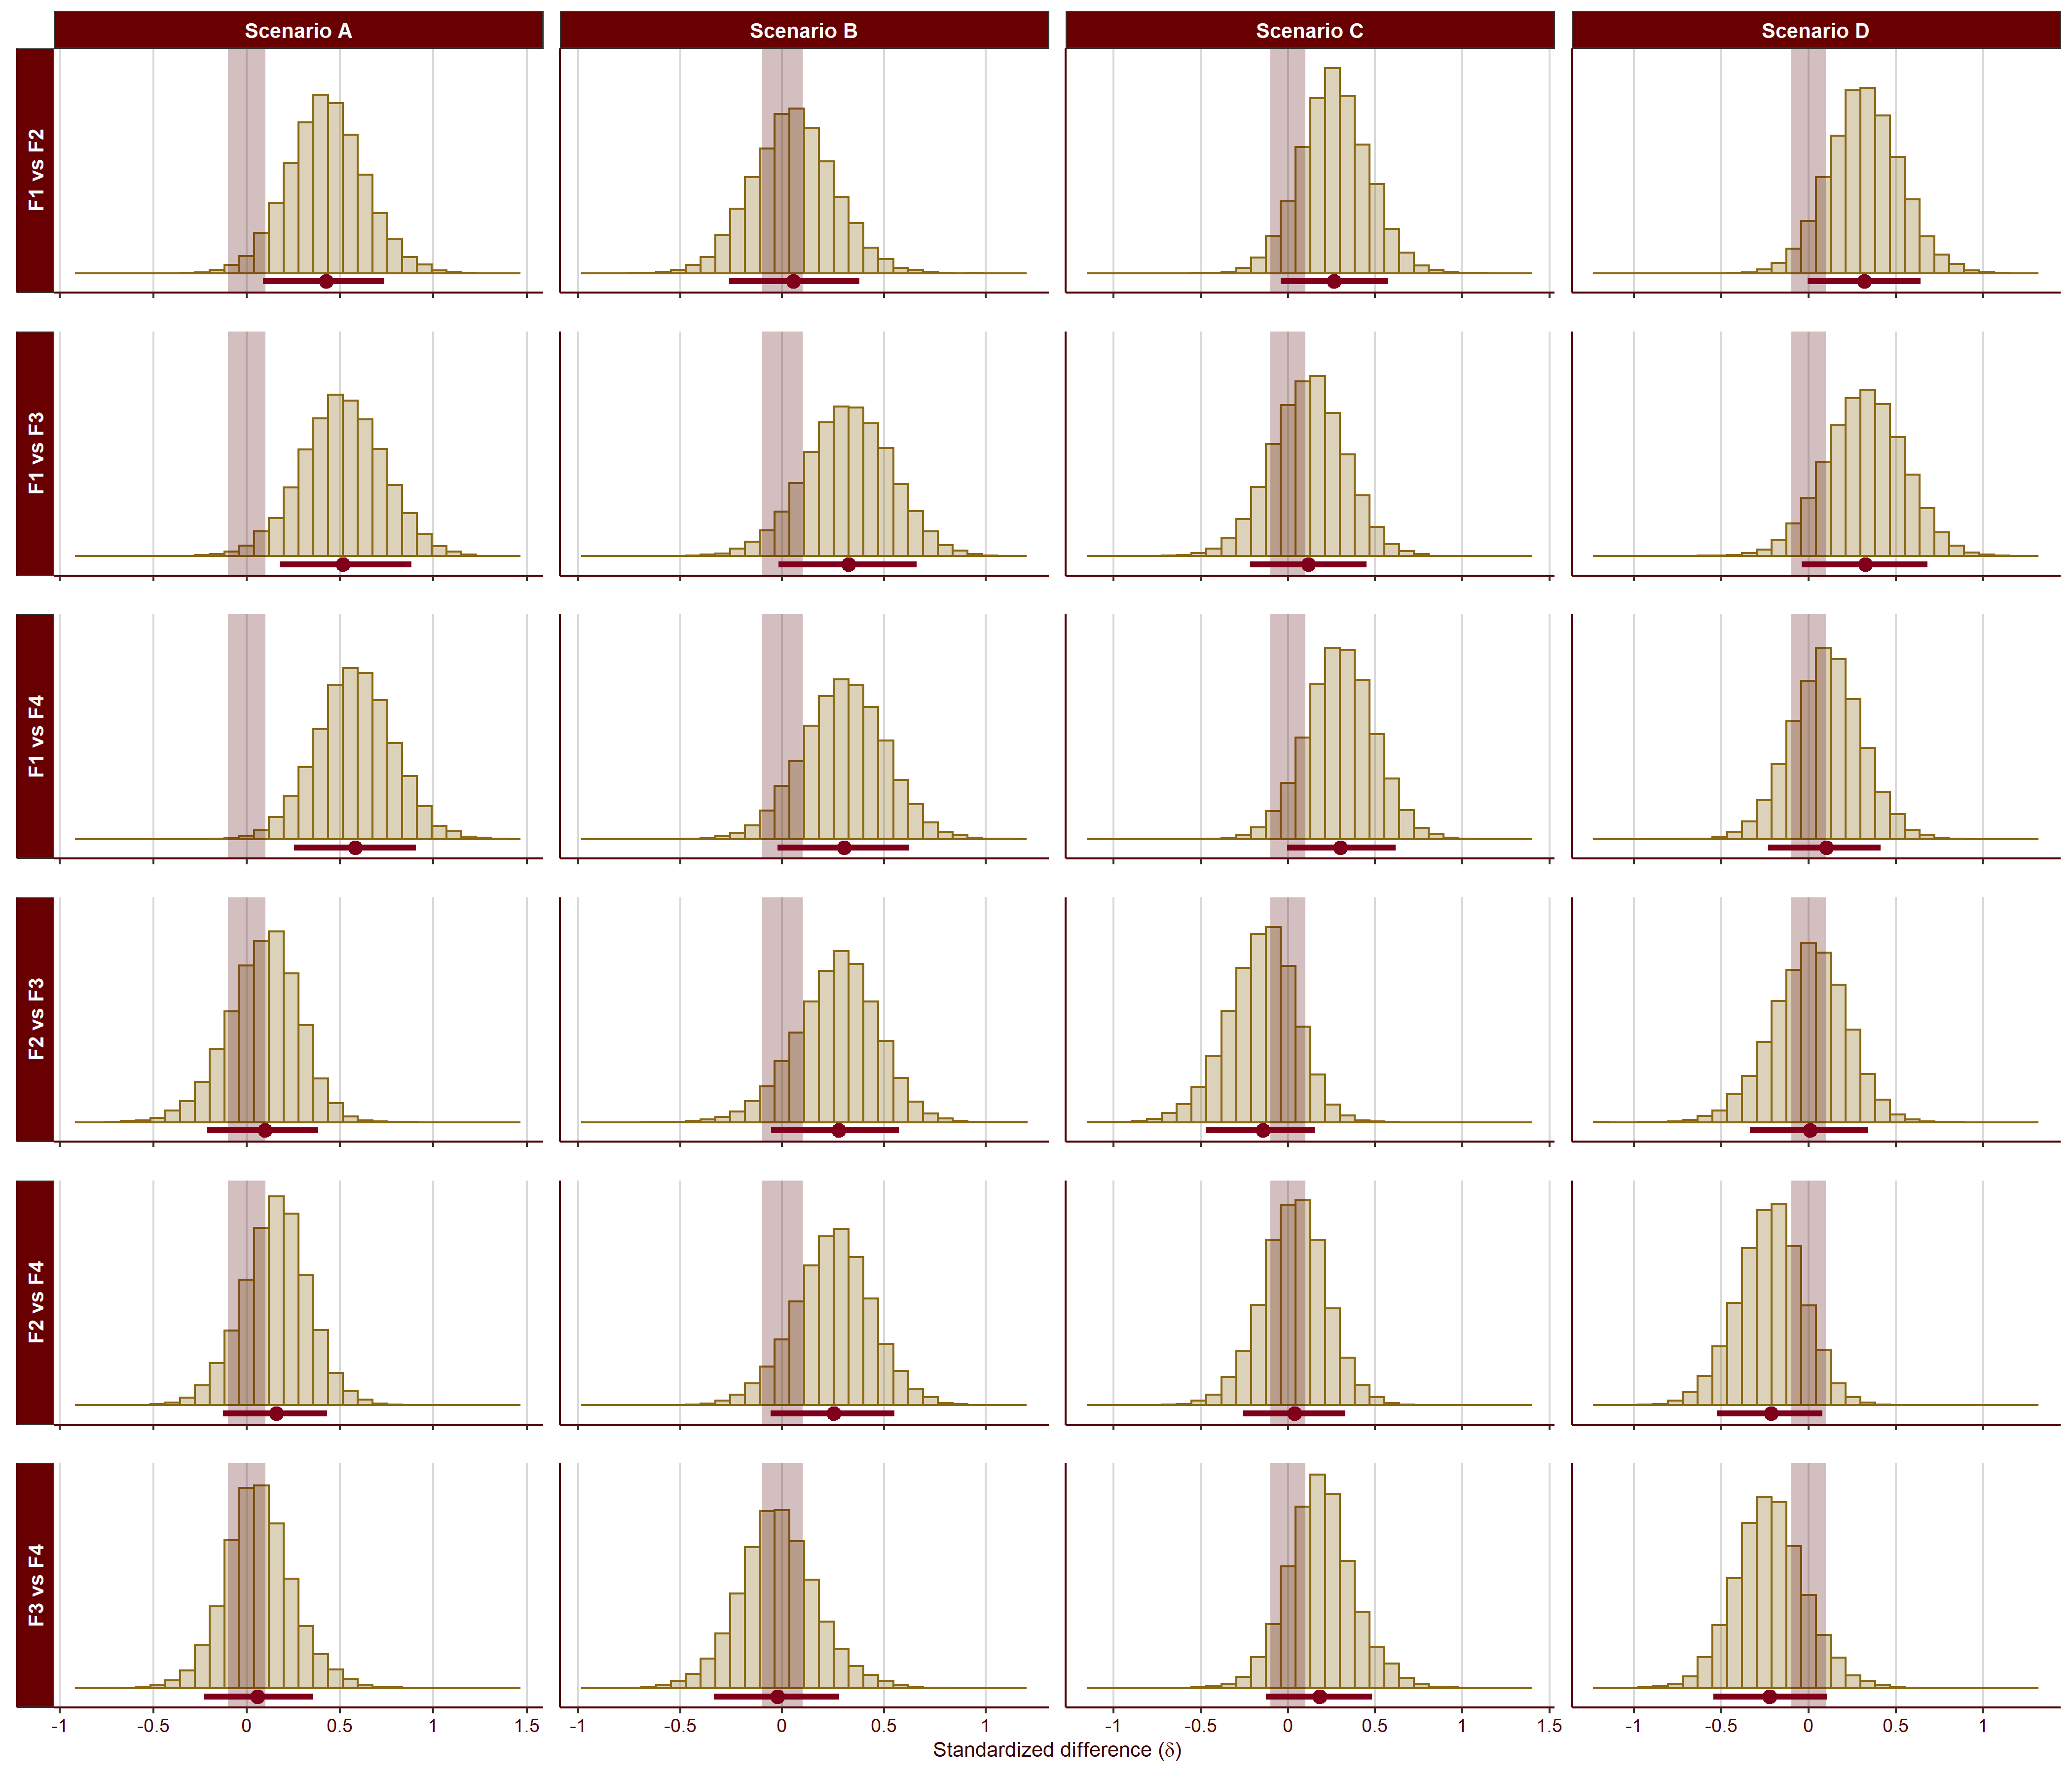
\includegraphics[width=\linewidth]{Figures/SD2_proportion_scenario_comparisons_C.png}
        \subcaption{Tallying}
        \label{fig:proportion-scenario-comparisons-C}
    \end{subfigure}
    \caption[]{Continued}
\end{figure}

\medskip

\begin{figure}[ht]\ContinuedFloat
    \centering
    \begin{subfigure}{1\textwidth}
        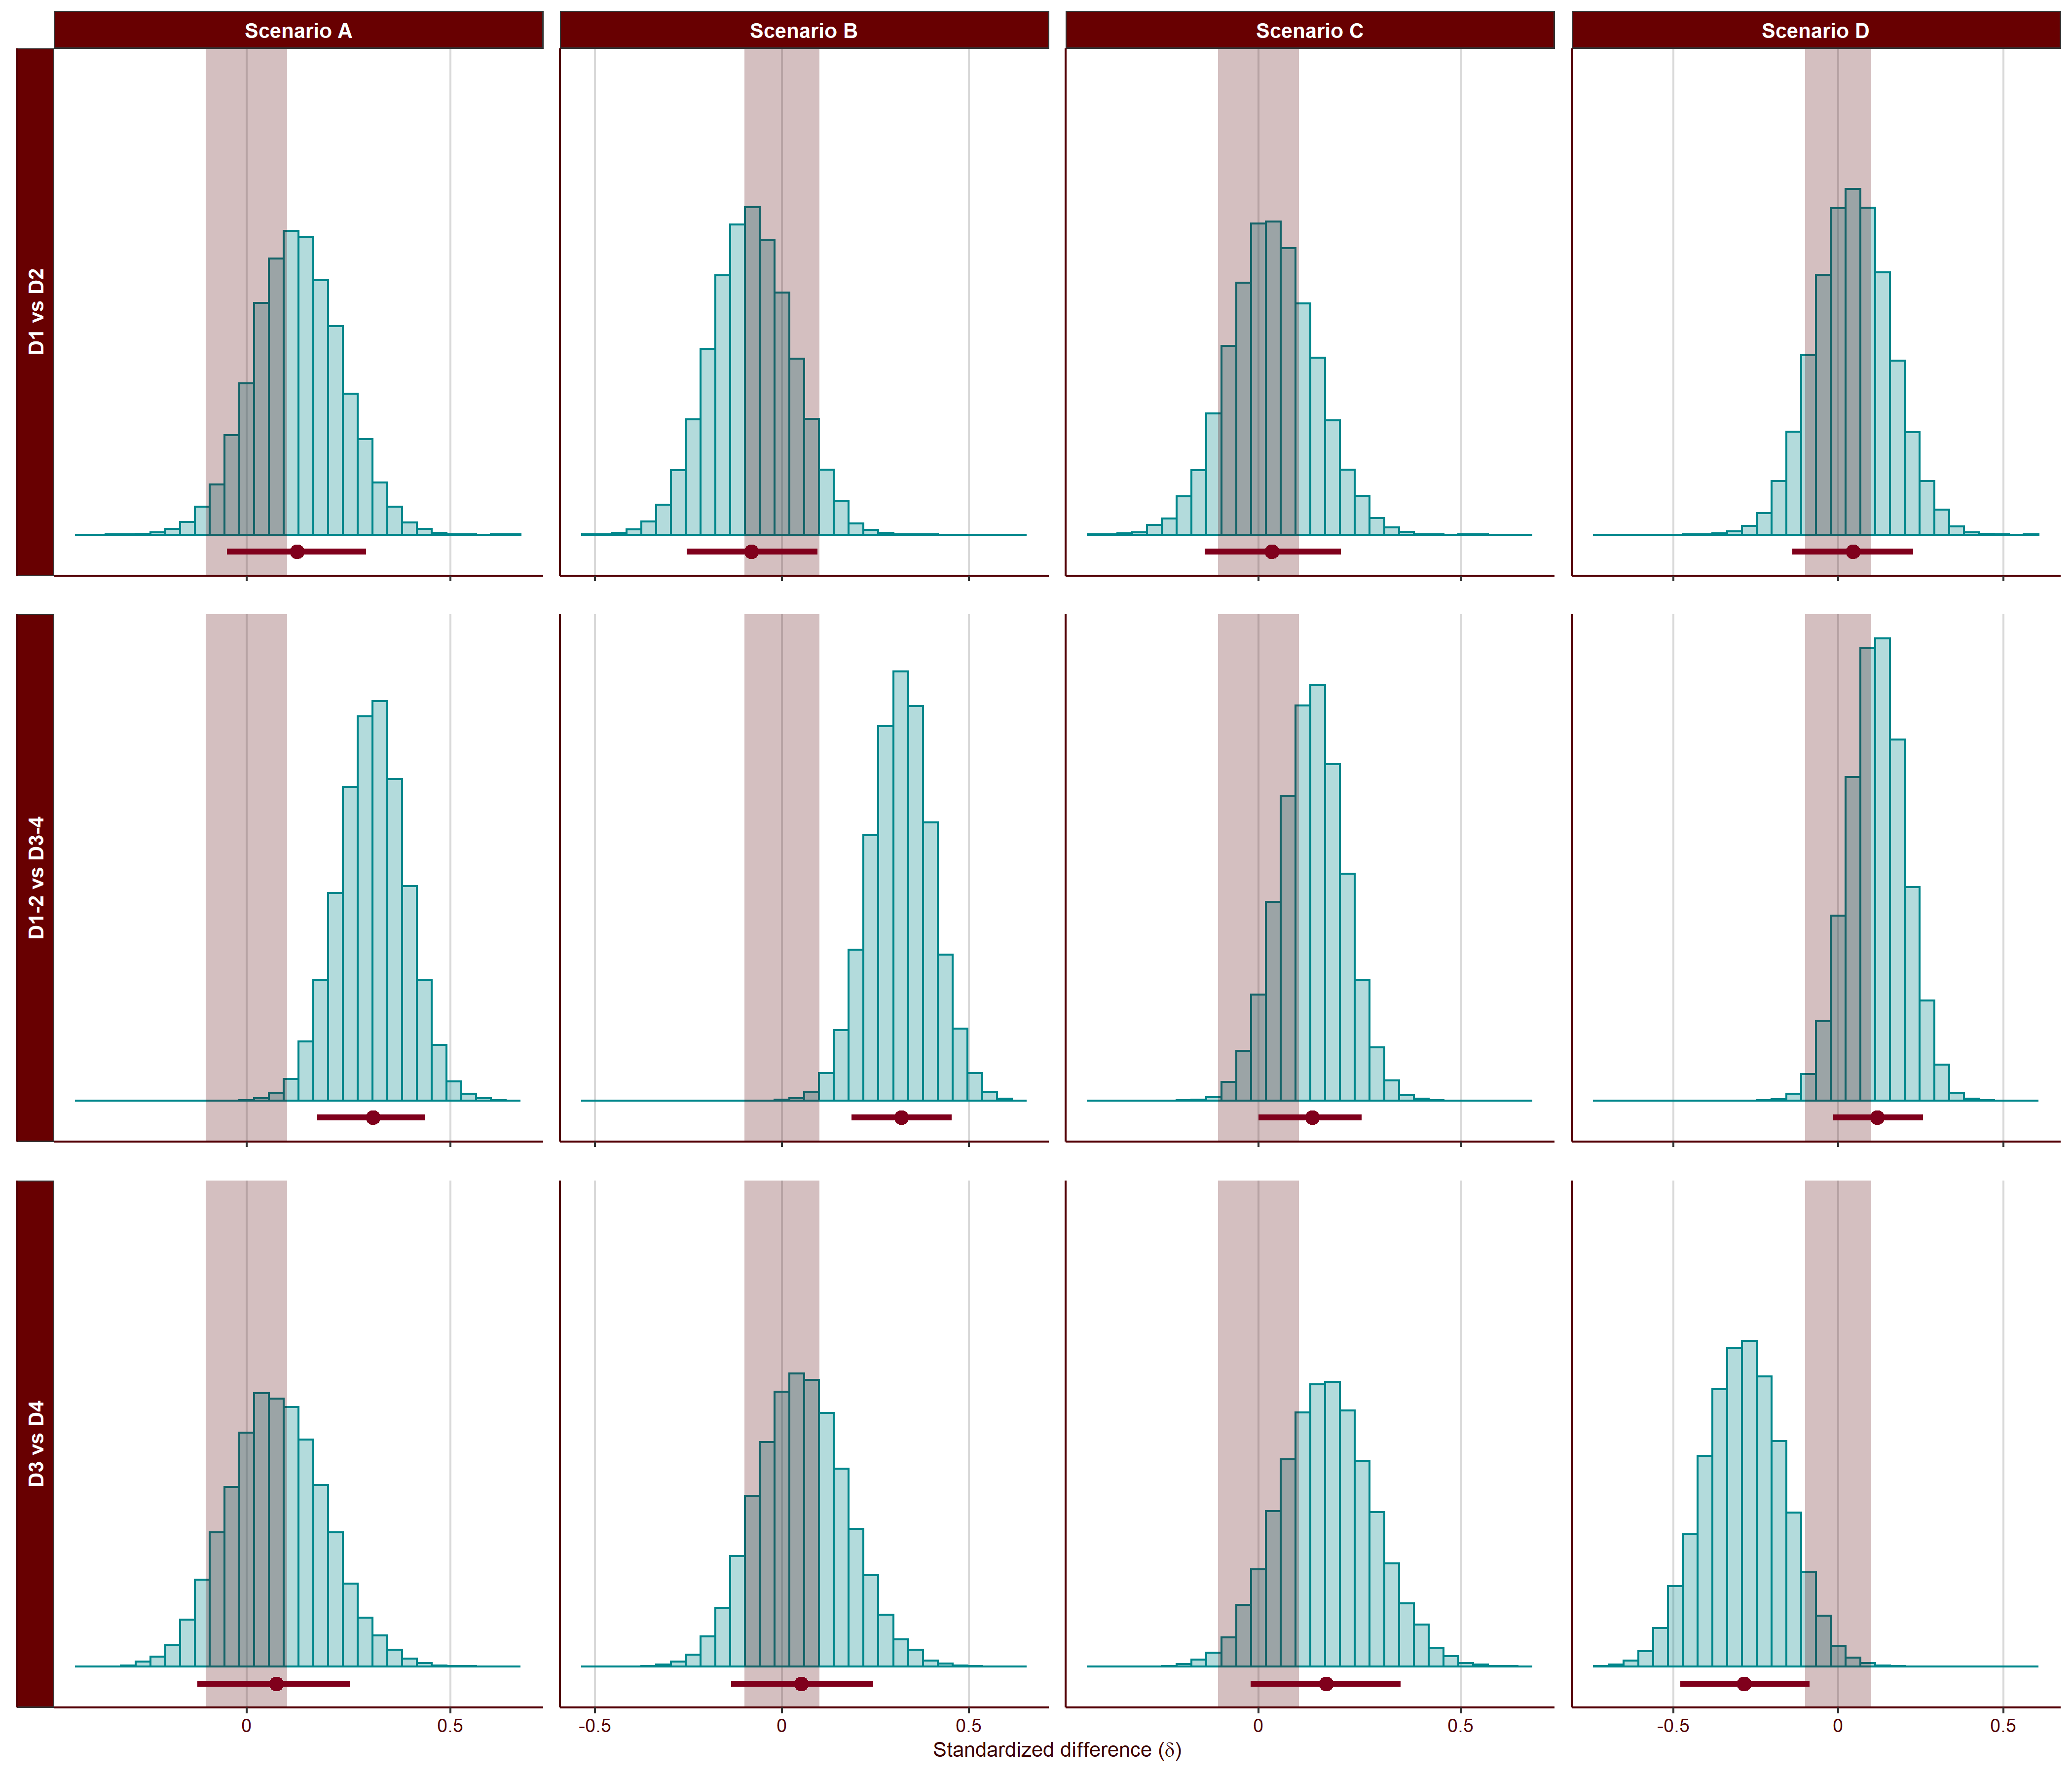
\includegraphics[width=\linewidth]{Figures/SD2_proportion_scenario_comparisons_D.png}
        \subcaption{Partial Tallying}
        \label{fig:proportion-scenario-comparisons-D}
    \end{subfigure}
    \caption[]{Continued}
    \label{fig:proportion-scenario-comparisons}
\end{figure}

\begin{figure}[!b]
    \centering
    \begin{subfigure}{1\textwidth}
        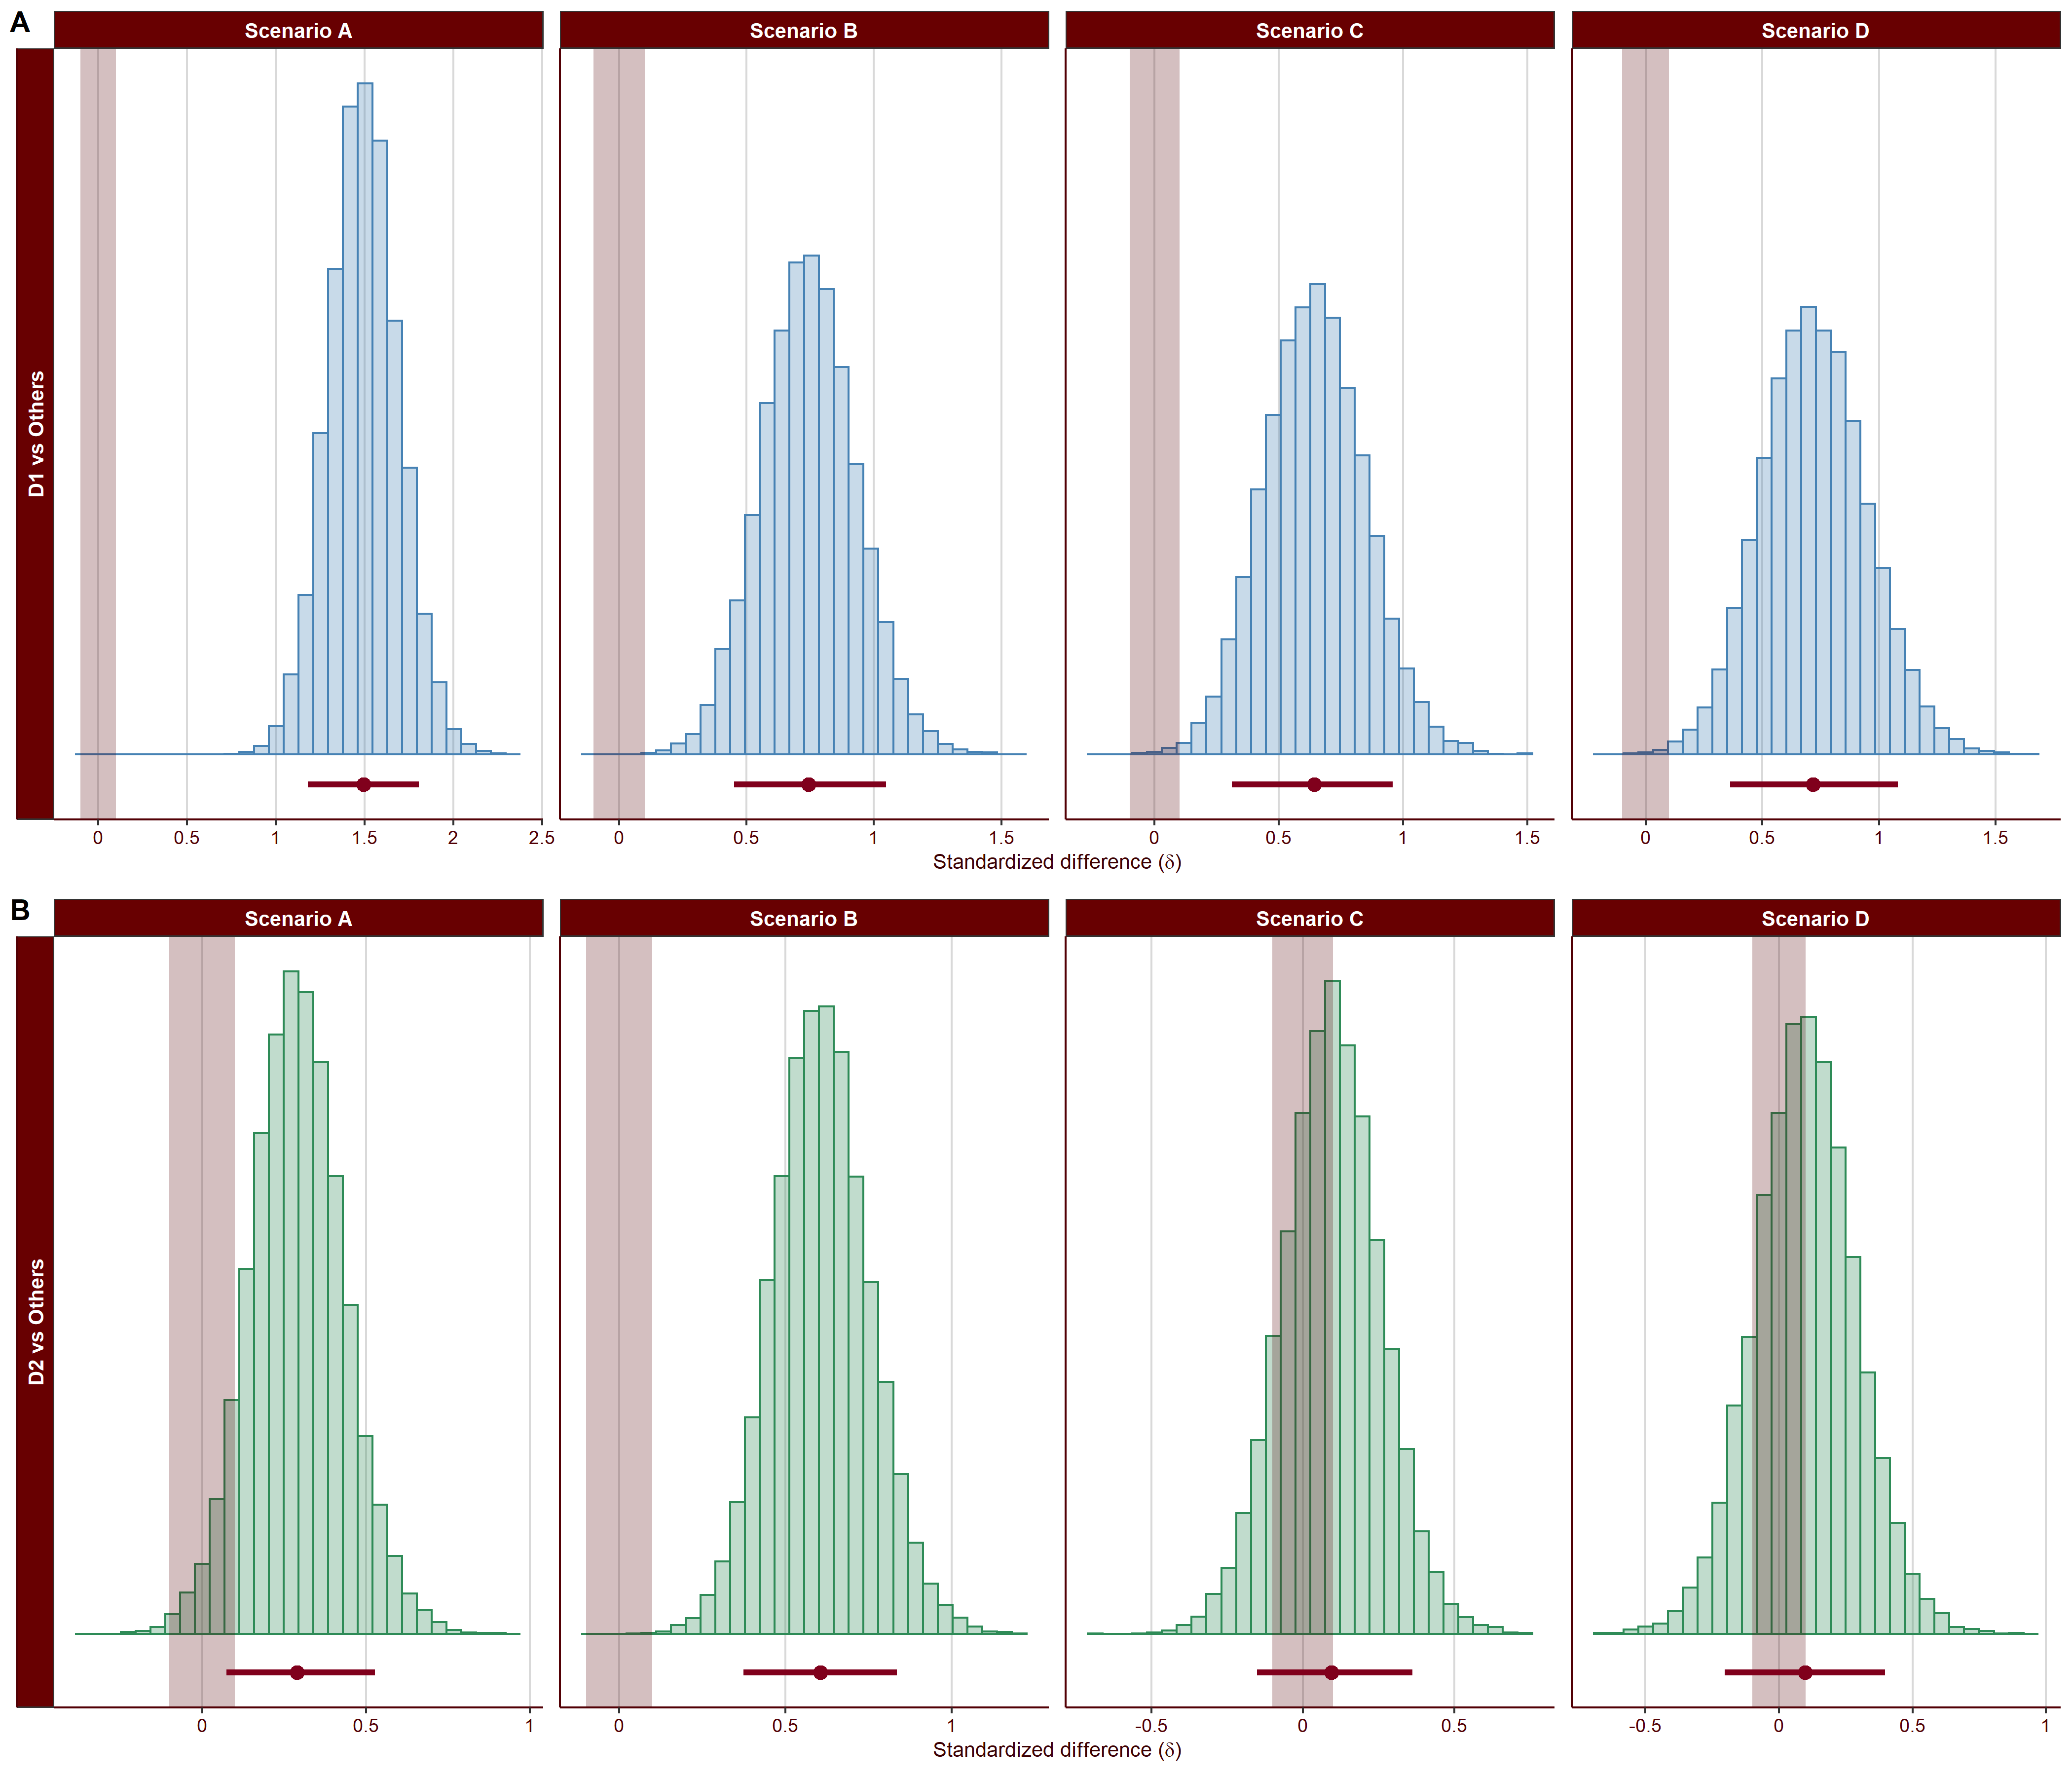
\includegraphics[width=\linewidth]{Figures/SE2_last_scenario_comparisons_A.png}
        \subcaption{1st only (A), 2nd only (B)}
        \label{fig:last-scenario-comparisons-A}
    \end{subfigure}
    \caption[]{Follow up comparisons for the allocation of last fixations across decision groups in the different decision scenarios. The horizontal red bar represents the 0.89 HDI. The shaded area highlights the ROPE used in these comparisons}
\end{figure}

\medskip

\begin{figure}[ht]\ContinuedFloat
    \centering
    \begin{subfigure}{1\textwidth}
        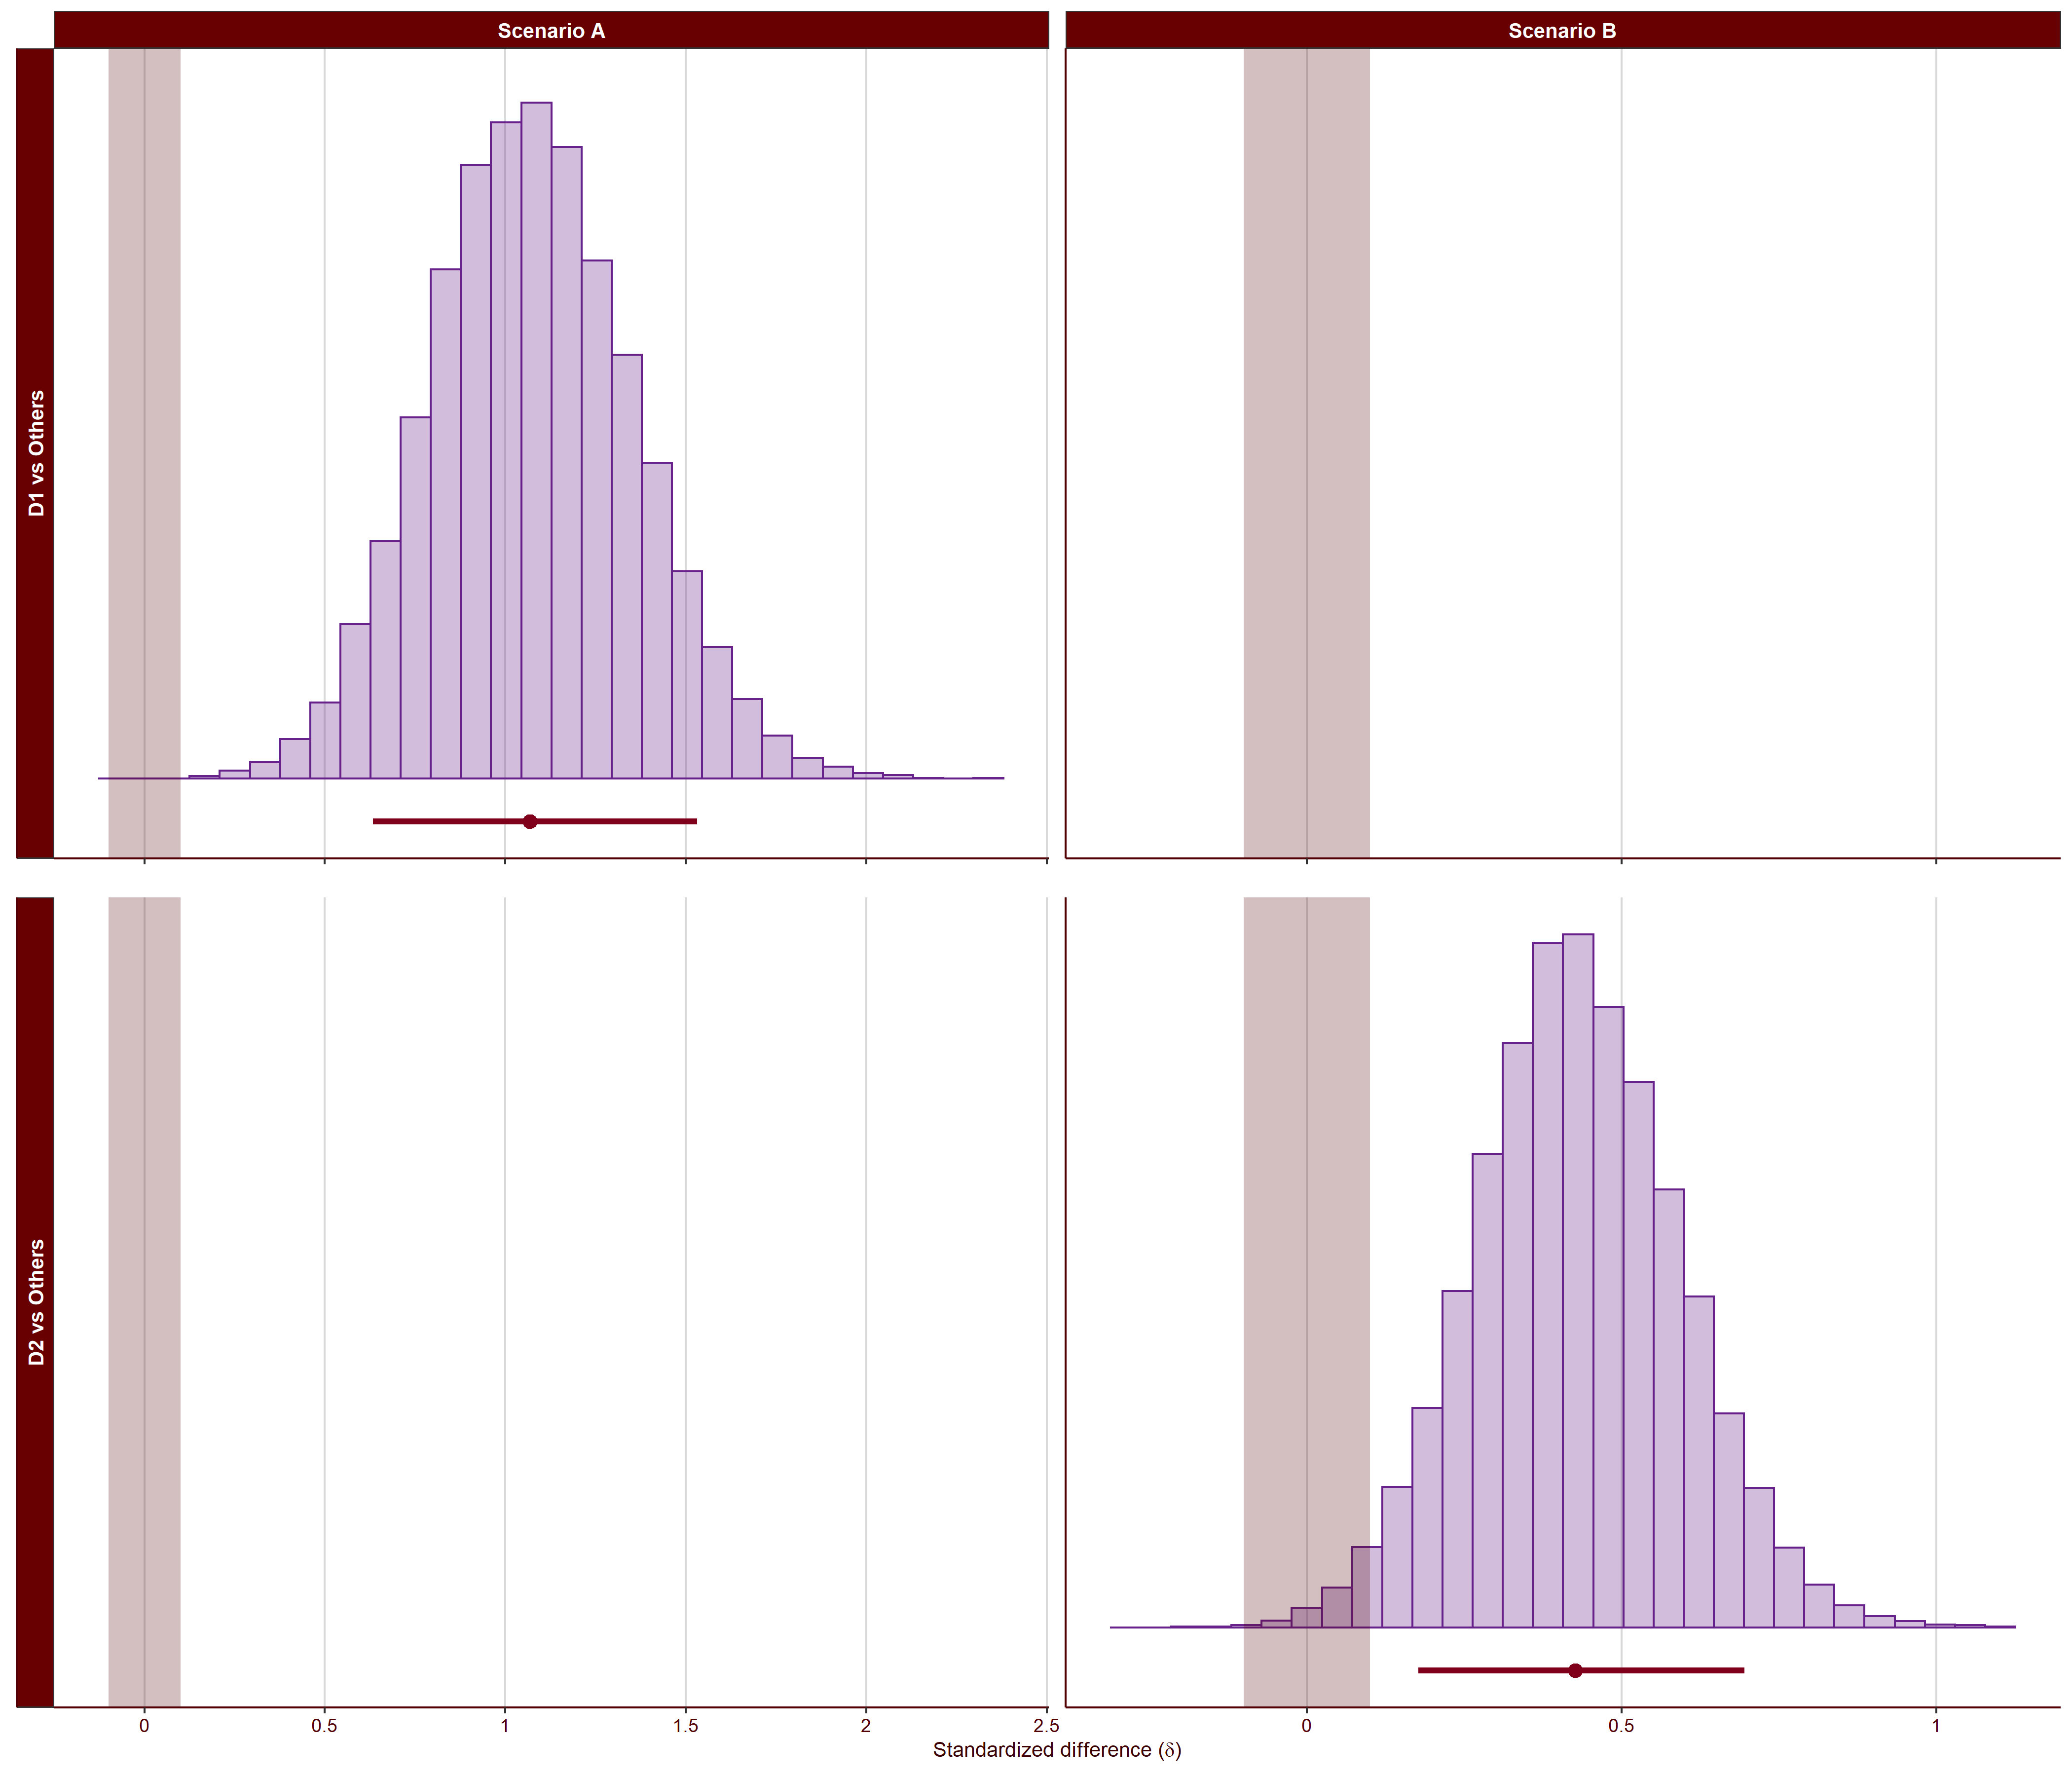
\includegraphics[width=\linewidth]{Figures/SE2_last_scenario_comparisons_B.png}
        \subcaption{Serial Search}
        \label{fig:last-scenario-comparisons-B}
    \end{subfigure}
    \caption[]{Continued}
\end{figure}

\medskip

\begin{figure}[ht]\ContinuedFloat
    \centering
    \begin{subfigure}{1\textwidth}
        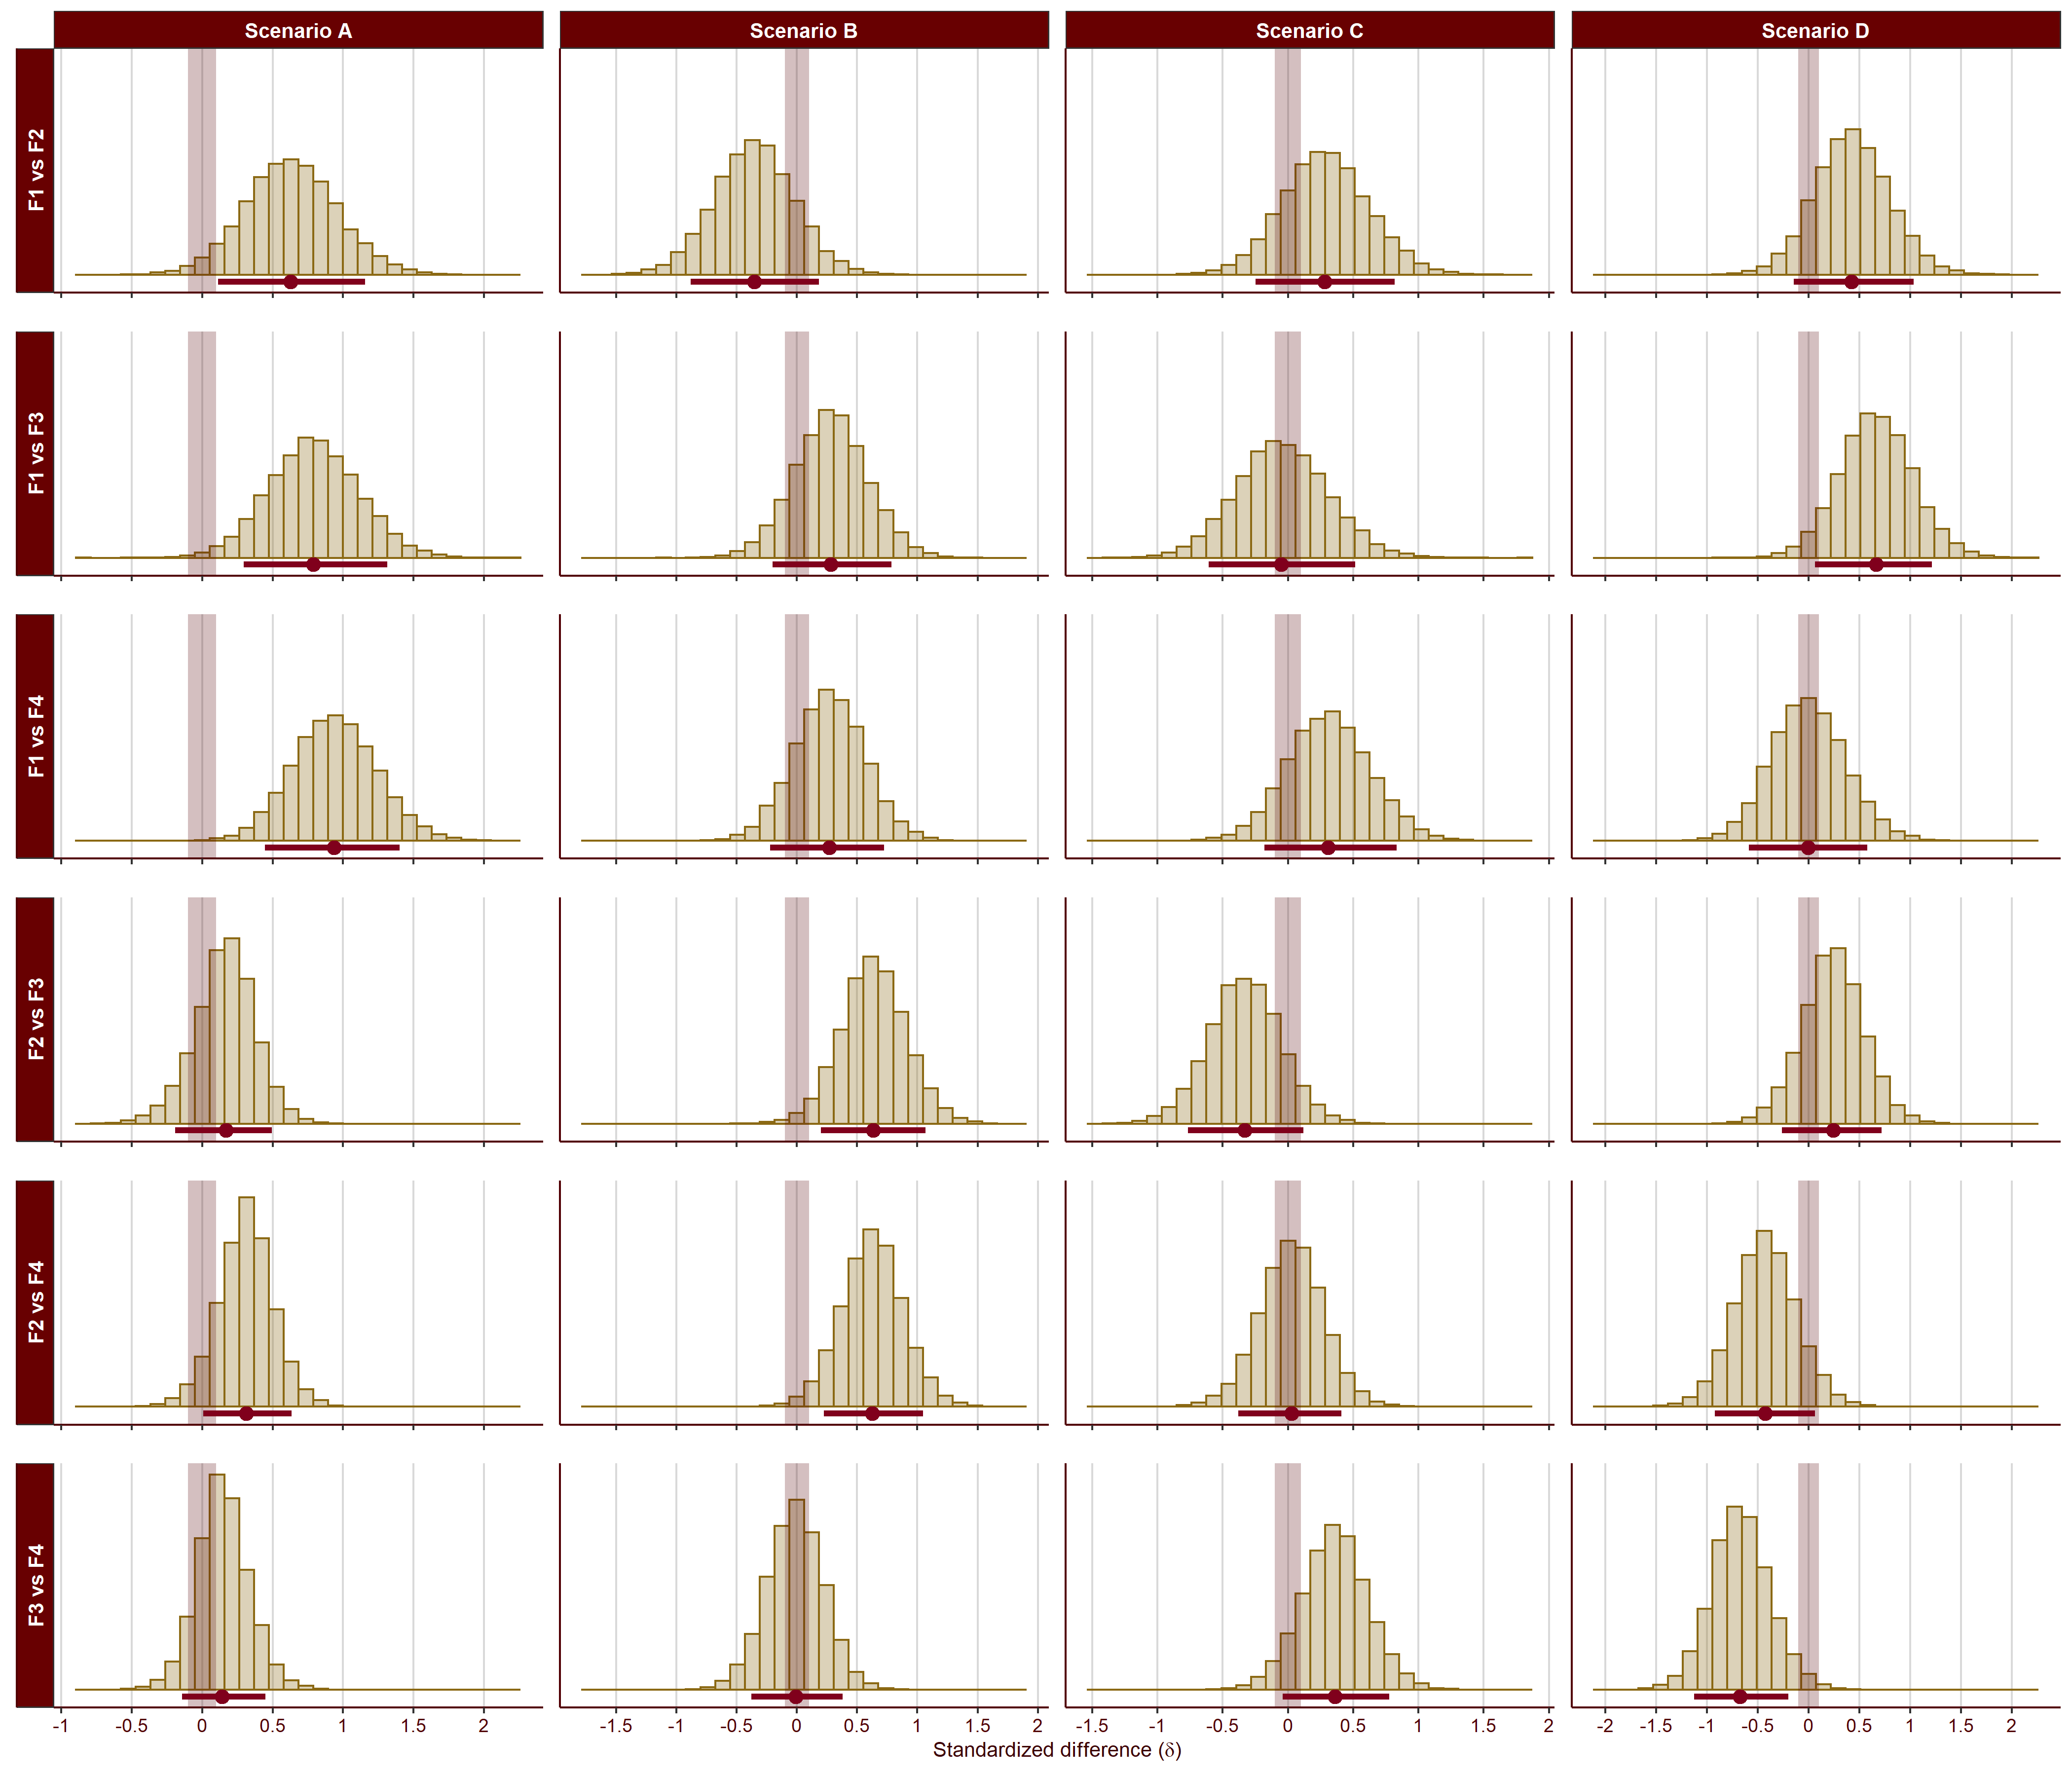
\includegraphics[width=\linewidth]{Figures/SE2_last_scenario_comparisons_C.png}
        \subcaption{Tallying}
        \label{fig:last-scenario-comparisons-C}
    \end{subfigure}
    \caption[]{Continued}
\end{figure}

\medskip

\begin{figure}[ht]\ContinuedFloat
    \centering
    \begin{subfigure}{1\textwidth}
        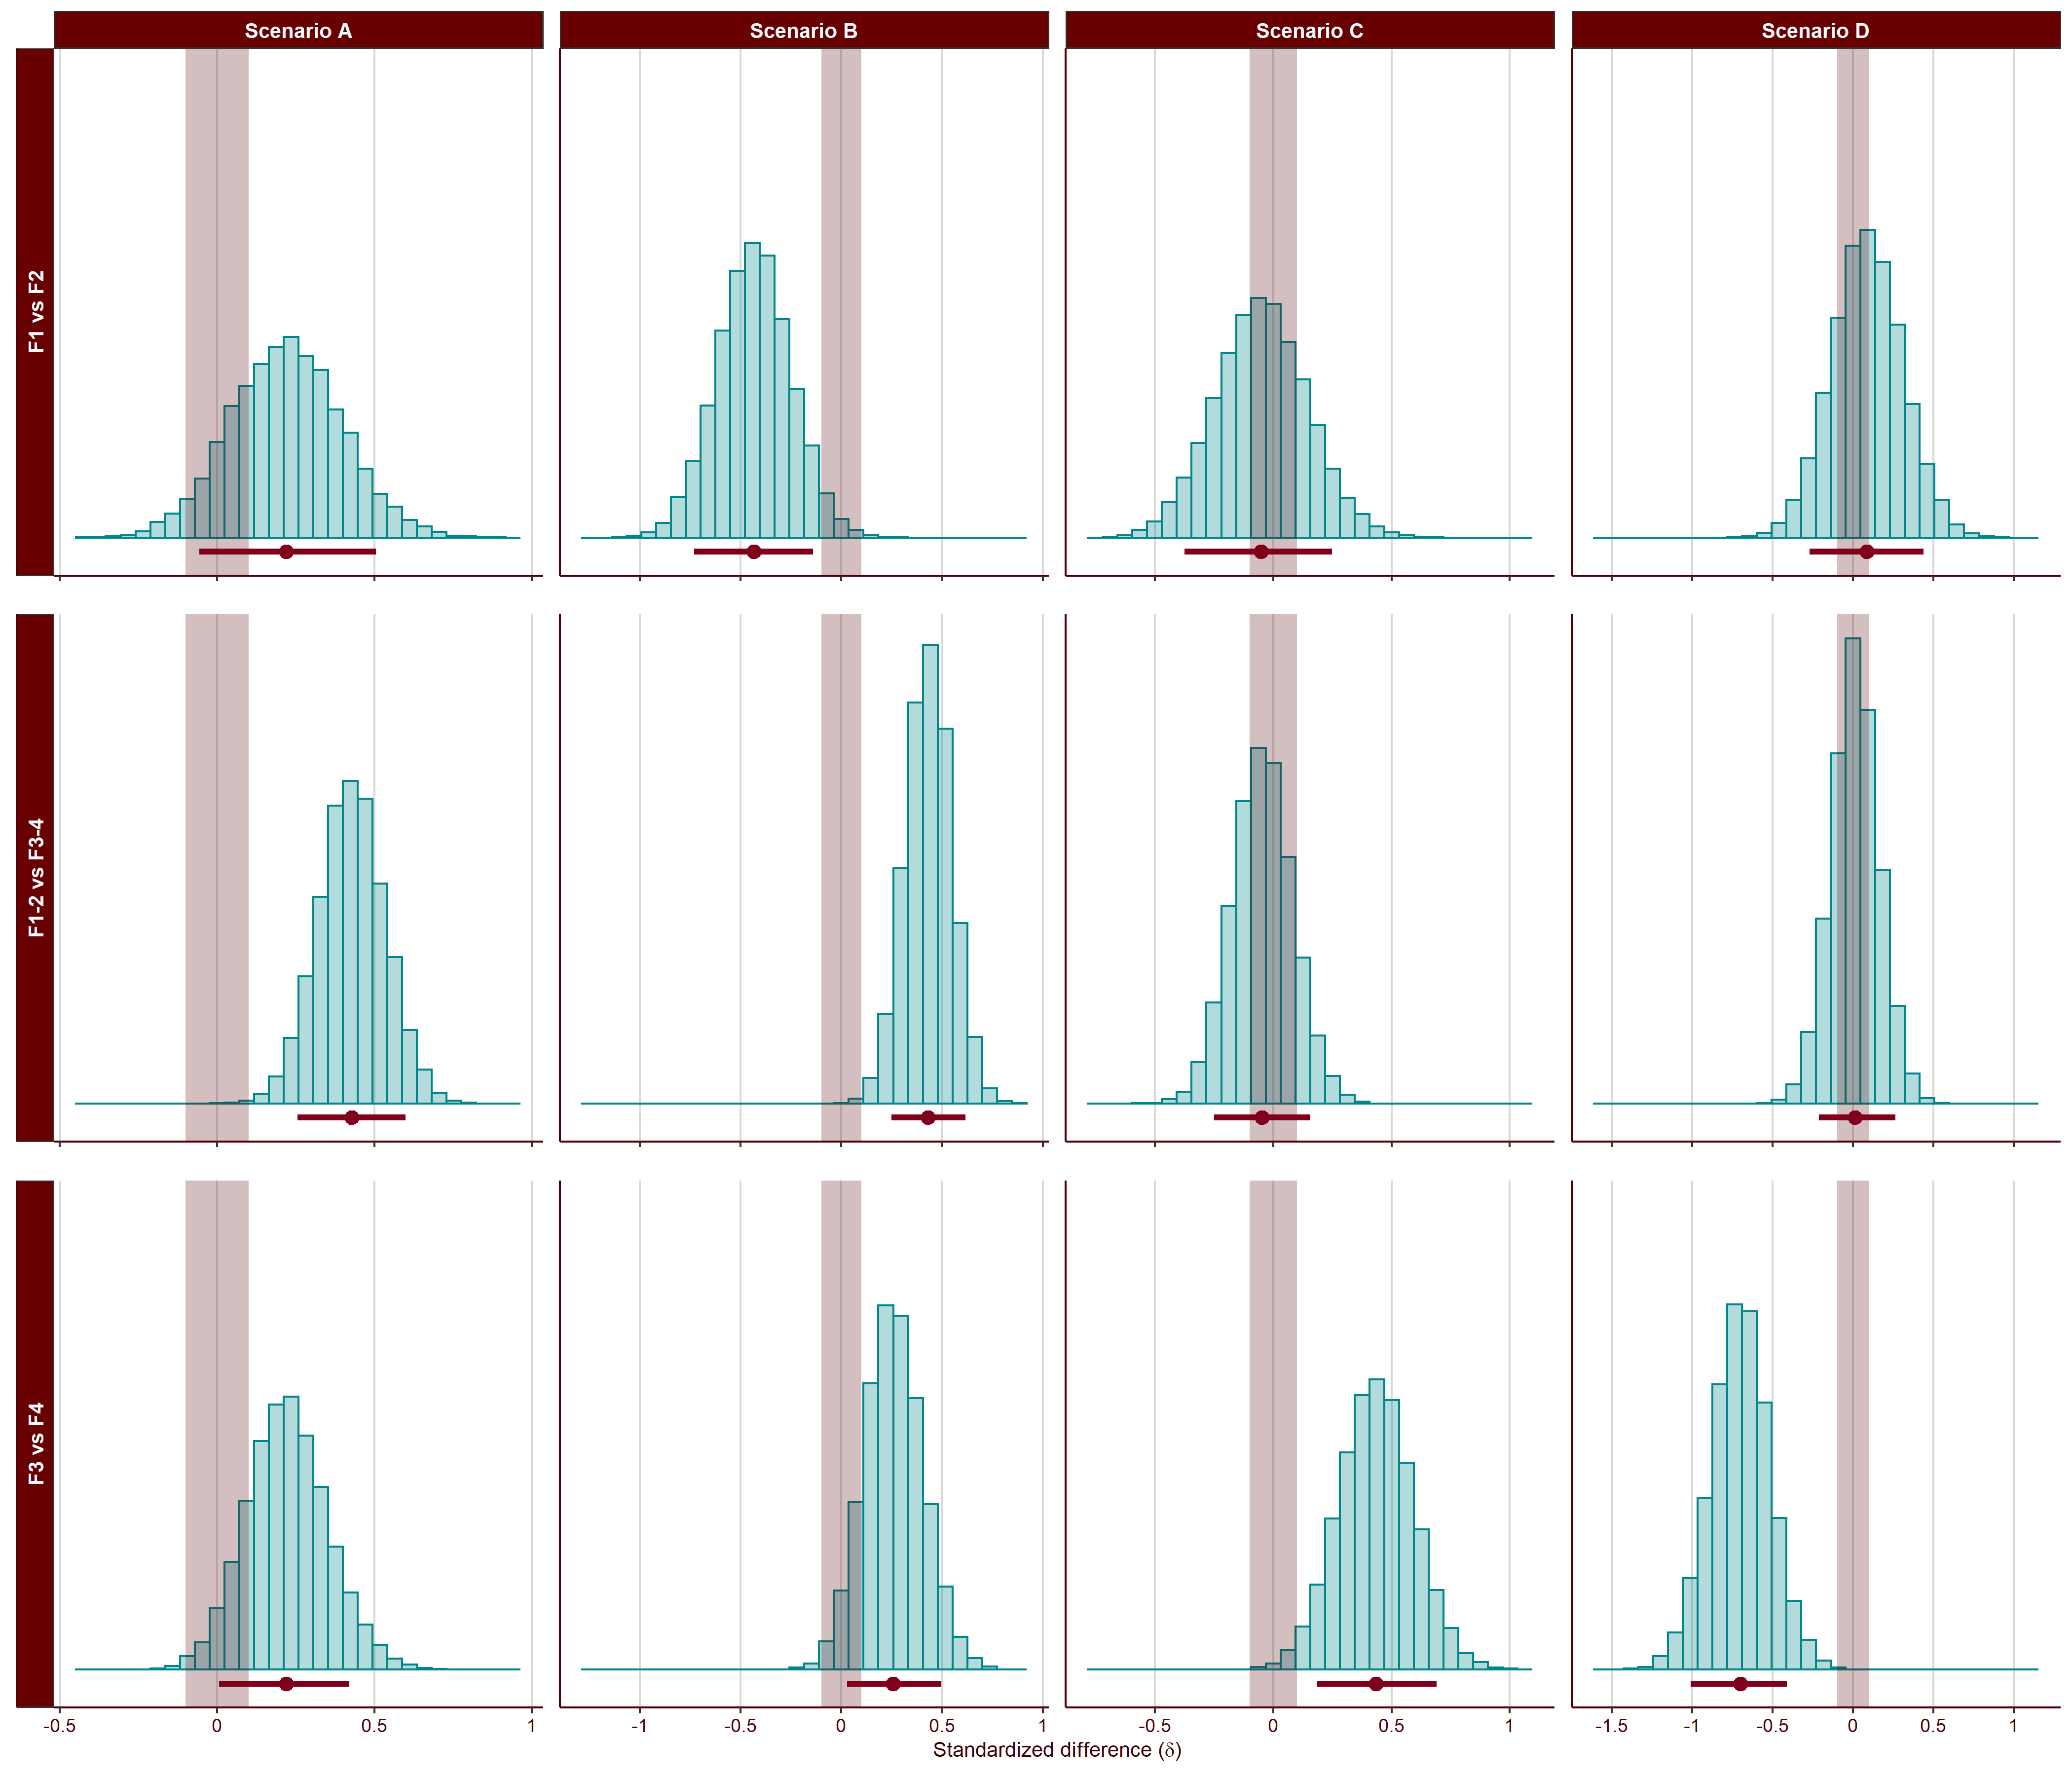
\includegraphics[width=\linewidth]{Figures/SE2_last_scenario_comparisons_D.png}
        \subcaption{Partial Tallying}
        \label{fig:last-scenario-comparisons-D}
    \end{subfigure}
    \caption[]{Continued}
    \label{fig:last-scenario-comparisons}
\end{figure}
\end{appendix}
